\documentclass[letterpaper]{article} % DO NOT CHANGE THIS
\usepackage[submission]{aaai2027}  % DO NOT CHANGE THIS
% The serif, sans-serif, and monospaced fonts are loaded automatically by
% aaai2027.sty (newtxtext, helvet, courier). DO NOT add \usepackage{times},
% \usepackage{helvet}, \usepackage{courier}, or any other font package.
\usepackage[hyphens]{url}  % DO NOT CHANGE THIS
\usepackage{graphicx} % DO NOT CHANGE THIS
\urlstyle{rm} % DO NOT CHANGE THIS
\def\UrlFont{\rm}  % DO NOT CHANGE THIS
\usepackage{natbib}  % DO NOT CHANGE THIS AND DO NOT ADD ANY OPTIONS TO IT
\usepackage{caption} % DO NOT CHANGE THIS AND DO NOT ADD ANY OPTIONS TO IT
\frenchspacing  % DO NOT CHANGE THIS
%
% These are recommended to typeset algorithms but not required. See the subsubsection on algorithms. Remove them if you don't have algorithms in your paper.
\usepackage{algorithm}
\usepackage{algorithmic}

%
% These are recommended to typeset listings but not required. See the subsubsection on listing. Remove this block if you don't have listings in your paper.
\usepackage{newfloat}
\usepackage{listings}
\DeclareCaptionStyle{ruled}{labelfont=normalfont,labelsep=colon,strut=off} % DO NOT CHANGE THIS
\lstset{%
	basicstyle={\footnotesize\ttfamily},% footnotesize acceptable for monospace
	numbers=left,numberstyle=\footnotesize,xleftmargin=2em,% show line numbers, remove this entire line if you don't want the numbers.
	aboveskip=0pt,belowskip=0pt,%
	showstringspaces=false,tabsize=2,breaklines=true}
\floatstyle{ruled}
\newfloat{listing}{tb}{lst}{}
\floatname{listing}{Listing}

%
% Recommended for better-looking tables
\usepackage{booktabs}
\usepackage{longtable}
% \usepackage[most]{tcolorbox}
% \usepackage{tcolorbox}
\usepackage{enumitem}
% \usepackage{listings}
% \tcbuselibrary{skins, breakable}
% \usepackage[utf8]{inputenc} % allow utf-8 input
% \usepackage[T1]{fontenc}    % use 8-bit T1 fonts
% \usepackage{url}            % simple URL typesetting
\usepackage{booktabs}       % professional-quality tables
\usepackage{amsfonts}       % blackboard math symbols
\usepackage{nicefrac}       % compact symbols for 1/2, etc.
\usepackage{microtype}      % microtypography
\usepackage{xcolor}         % colors
\usepackage{microtype}
\usepackage{graphicx}
\usepackage{subcaption}
\usepackage{booktabs} % for professional tables
\usepackage{amsmath}
\usepackage{amssymb}
\usepackage{mathtools}
\usepackage{amsthm}
% \usepackage{cleveref}

% \theoremstyle{plain}
% \newtheorem{theorem}{Theorem}[section]
% \newtheorem{proposition}[theorem]{Proposition}
% \newtheorem{lemma}[theorem]{Lemma}
% \newtheorem{corollary}[theorem]{Corollary}
% % \theoremstyle{definition}
% \newtheorem{definition}[theorem]{Definition}
% \newtheorem{assumption}[theorem]{Assumption}
% % \theoremstyle{remark}
% \newtheorem{remark}[theorem]{Remark}

\usepackage{multirow}
\usepackage{colortbl} % 用于设置表格颜色
\definecolor{lightblue}{RGB}{192,224,255} % 定义浅蓝色
\newcommand{\up}[1]{\textsubscript{\color{green!70!black}{↑#1}}}
\newcommand{\down}[1]{\textsubscript{\color{red!70!black}{↓#1}}}

\definecolor{bgblue}{RGB}{218, 232, 252}
\definecolor{bgpurple}{RGB}{225, 213, 231}
% \usepackage{amssymb}
\usepackage{pifont}
\usepackage[table]{xcolor}
\usepackage{fontawesome}
\newcommand{\cmark}{\textcolor{green!70!black}{\ding{51}}}
\newcommand{\xmark}{\textcolor{red!70!black}{\ding{55}}}
\newcommand{\pmark}{\textcolor{orange}{\ding{70}}} % ❖ 符号表示 Partial
\newcommand{\claw}{\textsuperscript{\small \faPaw}} % Claw 标识
\newcommand{\clawlogo}{\raisebox{-1pt}{\includegraphics[height=9pt]{claw.jpg}}}
%
% Keep the \pdfinfo as shown here. There's no need
% for you to add the /Title and /Author tags.
\pdfinfo{
/TemplateVersion (2027.1)
}

% DISALLOWED PACKAGES
% \usepackage{authblk} -- This package is specifically forbidden
% \usepackage{balance} -- This package is specifically forbidden
% \usepackage{CJK} -- This package is specifically forbidden
% \usepackage{float} -- This package is specifically forbidden
% \usepackage{flushend} -- This package is specifically forbidden
% \usepackage{fullpage} -- This package is specifically forbidden
% \usepackage{geometry} -- This package is specifically forbidden
% \usepackage{hyperref} -- This package is specifically forbidden
% \usepackage{navigator} -- This package is specifically forbidden
% (or any other package that embeds links such as navigator or hyperref)
% \usepackage{indentfirst} -- This package is specifically forbidden
% \usepackage{layout} -- This package is specifically forbidden
% \usepackage{multicol} -- This package is specifically forbidden
% \usepackage{nameref} -- This package is specifically forbidden
% \usepackage{savetrees} -- This package is specifically forbidden
% \usepackage{setspace} -- This package is specifically forbidden
% \usepackage{stfloats} -- This package is specifically forbidden
% \usepackage{tabu} -- This package is specifically forbidden
% \usepackage{titlesec} -- This package is specifically forbidden
% \usepackage{tocbibind} -- This package is specifically forbidden
% \usepackage{ulem} -- This package is specifically forbidden
% \usepackage{wrapfig} -- This package is specifically forbidden
% DISALLOWED COMMANDS
% \nocopyright -- Your paper will not be published if you use this command
% \addtolength -- This command may not be used
% \balance -- This command may not be used
% \baselinestretch -- Your paper will not be published if you use this command
% \clearpage -- No page breaks of any kind may be used for the final version of your paper
% \columnsep -- This command may not be used
% \newpage -- No page breaks of any kind may be used for the final version of your paper
% \pagebreak -- No page breaks of any kind may be used for the final version of your paper
% \pagestyle -- This command may not be used
% \tiny -- This is not an acceptable font size.
% \vspace{- -- No negative value may be used in proximity of a caption, figure, table, section, subsection, subsubsection, or reference
% \vskip{- -- No negative value may be used to alter spacing above or below a caption, figure, table, section, subsection, subsubsection, or reference

\setcounter{secnumdepth}{2} %May be changed to 1 or 2 if section numbers are desired.

% The file aaai2027.sty is the style file for AAAI Press
% proceedings, working notes, and technical reports.
%

% Title

% Your title must be in mixed case, not sentence case.
% That means all verbs (including short verbs like be, is, using,and go),
% nouns, adverbs, adjectives should be capitalized, including both words in hyphenated terms, while
% articles, conjunctions, and prepositions are lower case unless they
% directly follow a colon or long dash
% \title{Efficient In-Harness On-Policy Reinforcement Learning for Autonomous Agents}
% and Stable 
\title{Less Harness, More Signal: Efficient In-Harness RL for Autonomous Agents}

\author{
    %Authors
    % All authors must be in the same font size and format.
    Written by AAAI Press Staff\textsuperscript{\rm 1}\thanks{With help from the AAAI Publications Committee.}\\
    AAAI Style Contributions by Peter Patel Schneider,
    Sunil Issar,\\
    J. Scott Penberthy,
    George Ferguson,
    Hans Guesgen,
    Francisco Cruz\equalcontrib\corresponding,
    Marc Pujol-Gonzalez\equalcontrib\corresponding
}
\affiliations{
    %Afiliations
    \textsuperscript{\rm 1}Association for the Advancement of Artificial Intelligence\\
    % If you have multiple authors and multiple affiliations
    % use superscripts in text and roman font to identify them.
    % For example,

    % Sunil Issar\textsuperscript{\rm 2},
    % J. Scott Penberthy\textsuperscript{\rm 3},
    % George Ferguson\textsuperscript{\rm 4}\corresponding,
    % Hans Guesgen\textsuperscript{\rm 5}
    % Note that the comma should be placed after the superscript

    1101 Pennsylvania Ave, NW Suite 300\\
    Washington, DC 20004 USA\\
    % email address must be in roman text type, not monospace or sans serif
    proceedings-questions@aaai.org
%
% See more examples next
}

%Example, Single Author, ->> remove \iffalse,\fi and place them surrounding AAAI title to use it
\iffalse
\title{My Publication Title --- Single Author}
\author {
    Author Name
}
\affiliations{
    Affiliation\\
    Affiliation Line 2\\
    name@example.com
}
\fi

\iffalse
%Example, Multiple Authors, ->> remove \iffalse,\fi and place them surrounding AAAI title to use it
\title{My Publication Title --- Multiple Authors}
\author {
    % Authors
    First Author Name\textsuperscript{\rm 1,\rm 2}\equalcontrib,
    Second Author Name\textsuperscript{\rm 2}\equalcontrib,
    Third Author Name\textsuperscript{\rm 1}\corresponding
}
\affiliations {
    % Affiliations
    \textsuperscript{\rm 1}Affiliation 1\\
    \textsuperscript{\rm 2}Affiliation 2\\
    firstAuthor@affiliation1.com, secondAuthor@affilation2.com, thirdAuthor@affiliation1.com
}
\fi

\begin{document}
\maketitle

\begin{abstract}
In-harness reinforcement learning (RL), where each rollout executes within a live environment (e.g., OpenClaw), has become essential for training autonomous LLM-based agents.
% capable of multi-turn tool use and long-horizon planning. 
However, repurposing such harnesses for RL training introduces two critical bottlenecks:
(1)~environment execution dominates per-episode wall-clock time, severely underutilizing GPU resources; 
and (2)~trajectory-level credit assignment in standard RL algorithms reinforces ineffective interactions alongside productive steps, leading to suboptimal policy convergence in autonomous tasks. 
We address both issues in a unified framework. 
On the systems side, we propose \textit{ClawLoop}, a lightweight white-box training harness that strips non-essential product components while retaining a minimal five-element interaction loop.
This design reduces environment overhead by $8.8\times$ and lifts GPU utilization from 14\% to 49\%. 
Building on this infrastructure, we propose \emph{Asymmetric Advantage Masking} to resolving the credit misassignment problem in RL.
It is a token-level correction mechanism that selectively suppresses spurious positive gradients on ineffective actions while preserving negative signals. 
Experiments across five benchmarks and model scales from 2B to 27B parameters show that our framework eliminates training collapse, improves success rate by up to $+7.8$ points over the base model, matches frontier proprietary models at 27B scale, and reduces inference-time token consumption by 32\%.
% Experiments across five benchmarks and model scales ranging from 2B to 27B parameters demonstrate that our framework eliminates training collapse, improves success rates by up to $+7.8$ points over the base model, matches frontier proprietary models at the 27B scale, and reduces inference-time token consumption by 32\%.

\end{abstract}

% Uncomment the following to link to your code, datasets, an extended version or similar.
% You must keep this block between (not within) the abstract and the main body of the paper.
% Make sure that you do not de-anonymize yourself with these links.
% \begin{links}
%     \link{Code}{https://aaai.org/example/code}
%     \link{Datasets}{https://aaai.org/example/datasets}
%     \link{Extended version}{https://aaai.org/example/extended-version}
% \end{links}

% todo intro中 绘制一个图, 表示 in-harness RL 时间开销, 与Automous Agent 训练崩溃问题.

\section{Introduction}
% % P1： OpenClaw 与 Agent Harness 背景
% % 随着自主智能体（Autonomous Agents）的快速发展，大语言模型（LLM）正从被动的文本生成器转向主动、基于工具调用的问题解决者。
% % todo add 什么是Autonomous Agents? 长程, 多轮, 工具调用能力. Harness 是可以end to end 落地释放这种能力的底层执行基础设施.
% % 它集成了沙箱运行环境、自动化可观测性与动态反馈闭环。其中OpenClaw, Hermes-Agent, Claude-Code, Codex 是代表性的harness.
% % In contrast to single-turn question answering, such an agent pursues complex objectives over long horizons and multiple interaction turns, autonomously planning and invoking external tools in an iterative loop until the goal is achieved. 
LLMs are evolving from passive text generators into proactive, tool-using problem solvers, i.e., \emph{autonomous agents} that pursue complex goals over long, multi-turn horizons by iteratively planning and invoking external tools~\citep{lopopolo2026harness}. 
Delivering this ability end to end requires an \emph{execution harness}: low-level infrastructure that grounds the agent in a runnable environment through a sandboxed runtime, automated observability, and a dynamic feedback loop. 
Representative harnesses include OpenClaw~\citep{openclaw}, Hermes-Agent~\citep{nousresearch2026hermes}, Claude Code~\citep{claudecode}, and Codex~\citep{openai2025codex}.

% % P2：Claw-style Agent 的特殊性与训练必要性
Unlike traditional tasks, Claw-style tasks operate over long-horizon trajectories involving multi-turn tool calling, interactive trial-and-error, and continuous environmental state transitions. 
Training such agents has progressed from supervised fine-tuning on synthesized trajectories~\citep{bai2026clawgym,xia2026metaclaw} to on-policy RL executed directly inside the harness~\citep{xu2026polar,wang2026openclaw}, where each rollout interleaves model generation with real environment feedback and is scored by an external verifier.
This \emph{in-harness RL} recipe is essential: only by closing the loop over live tools can the policy acquire multi-turn planning, error recovery, and state-tracking capabilities that static distillation cannot provide.
However, repurposing product-grade harnesses as RL training environments introduces new bottlenecks (as shown in Fig. \ref{fig:intro}), rendering training both prohibitively slow and fundamentally unstable. 

% % P3：现有训练路线及其核心开销瓶颈
The first bottleneck is \emph{environment overhead}. Product harnesses are engineered for end-user functionality
% , persistent sessions, plugin registries, authentication, multi-agent orchestration, 
rather than for high-throughput gradient estimation. 
We quantify this gap via a controlled comparison (\S\ref{subsec:prelim_cost}): under a full OpenClaw harness, environment execution consumes 94\% of per-episode wall-clock time (54.1\,s), making in-harness rollouts $9.7\times$ slower than a tool-only baseline on the \emph{same} task. 
Crucially, the bottleneck is not GPU-bound: GPU utilization collapses from 61\% to 14\% because the accelerator idles while the system waits on CPU/IO-bound sandbox interactions. 
% Adding GPUs cannot resolve an architectural latency problem; 
Addressing this necessitates a training-oriented harness that strips product-level complexity while retaining the minimal interaction loop required for policy gradient computation.

The second bottleneck is \emph{credit misassignment}. 
Standard on-policy RL algorithms (e.g., GRPO~\citep{guo2025deepseek}) broadcasts a trajectory-level advantage to every generated token. 
In long-horizon tasks, a trajectory may succeed despite containing ineffective interactions, e.g., truncated turns and action errors. 
Because the sparse binary reward cannot distinguish productive steps from wasted ones, positive gradient reinforces both indiscriminately.
We show empirically (\S\ref{subsec:prelim_misassign}) that the fraction of positive learning signal landing on ineffective tokens, $\psi_+$, surges from 0.04 in early training to 0.20 after the performance peak, at which point the success rate \emph{collapses}: the policy has learned to reproduce lucky-but-inefficient behavior.
% This failure is not a reward-design flaw---the verifier remains well-defined throughout---but a structural consequence of uniform credit assignment over long, heterogeneous trajectories.
% The verifier remains well-defined throughout; the failure stems entirely from broadcasting a coarse, trajectory-level signal over long, heterogeneous trajectories.

We address both bottlenecks in a unified framework.
On the systems side, we introduce \textit{ClawLoop}, a lightweight, white-box training harness reconstructed from OpenClaw by removing all non-essential product components (e.g., gateway, plugin registries, background services) and retaining a minimal five-element closed loop:
task specification, environment state, tool execution, multi-turn interaction, and terminal verification. 
It exposes token-level log-probabilities and structured rollout records, enabling direct policy-gradient computation without parsing external APIs, and integrates as a thin environment interface into the VERL distributed RL system~\citep{sheng2024verl}.
On the algorithmic side, we propose \textit{Asymmetric Advantage Masking (AAM)}, a token-level correction that identifies ineffective interactions via four deterministic environment-side rules and suppresses their gradient contribution \emph{only when the advantage is positive}. 
Negative advantages are preserved, so the policy continues to receive penalization signals for failed trajectories. 
% Crucially, the mask is advantage-conditioned: when the same ineffective tokens appear in a \emph{failed} trajectory (negative advantage), their gradient is preserved, allowing the policy to actively learn avoidance rather than merely forgetting the behavior.

Experiments on five benchmarks, including three in-domain Claw-style tasks (PinchBench, ClawEval, ClawBenchPro) and two out-of-domain tool-use settings (BFCL-v3, $\tau^2$-bench), demonstrate consistent gains across model scales from 2B to 27B parameters.
On the efficiency side, ClawLoop achieves an $8.8\times$ reduction in per-episode environment time and lifts GPU utilization from 14\% to 49\%. 
On the training side, AAM eliminates the training collapse observed under standard GRPO, improving success rate by $+5.1$ points over
GRPO and $+7.8$ points over the base model on Qwen3.5-9B.
At the 27B scale, AAM-trained agents match frontier proprietary models (e.g., GPT-5.4) on in-domain harness tasks.
At inference time, AAM further reduces per-episode token consumption by 32\% on Qwen3.5-9B while maintaining competitive accuracy,
confirming that correcting credit misassignment yields not only more accurate but also more efficient agent behavior.

% In summary, our main contributions are:
% \begin{itemize}[nosep,leftmargin=*]
%     \item We identify and quantify two critical bottlenecks in in-harness agent RL: prohibitive environment overhead and credit misassignment leading to training collapse.
%     \item We develop {ClawLoop}, a lightweight white-box harness that strips product-level complexity, accelerating environment execution by $8.8\times$.
%     \item We propose {asymmetric advantage masking} strategy, a token-level correction that eliminates training collapse, yielding consistent accuracy and efficiency gains across scales and benchmarks.
% \end{itemize}

\section{Related Works}

\paragraph{Agent Harness.}
Agent harnesses provide the execution infrastructure, integrating sandboxes, observability, and feedback loops, that mediates interactions between LLMs and external environments \citep{lopopolo2026harness}. 
Pioneered by domain-specific orchestrators like Claude Code \citep{anthropic2025claudecode} and Codex \citep{openai2025codex} in software engineering, harnesses have evolved into general-purpose frameworks such as OpenClaw \citep{steinberger2026openclaw}, NanoClaw \citep{nanoclaw2026}, and Hermes-Agent \citep{nousresearch2026hermes} to support open-ended tasks. 
To measure these capabilities, benchmarks within the Claw-style ecosystem, including PinchBench \citep{kiloaiteam2026pinchbench} and Claw-Eval \citep{ye2026claw}, evaluate agents across coding, web interaction, and autonomous research workflows.

\paragraph{Claw-style Agent Training.}
Recent advances in Claw-style agent training can be categorized into two paradigms. 
The first paradigm relies on trajectory synthesis and SFT \citep{bai2026clawgym, li2026clawenvkit, xia2026metaclaw}. 
For instance, ClawGym \citep{bai2026clawgym} generates large-scale executable tasks and collects high-fidelity trajectories via black-box rollouts. 
The second paradigm employs On-Policy Distillation (OPD) to acquire long-horizon task-solving capabilities from teacher models \citep{wang2026openclaw, yang2026nemotron, bai2026scaling}; e.g., OpenClaw-RL \citep{wang2026openclaw} optimizes policies online by extracting instructional signals from interactive environments. 
However, both approaches are fundamentally bottlenecked—either capped by static trajectory or teacher.

To break these limitations, in-harness RL pushes this performance ceiling \citep{yue2025does,guo2025deepseek}. 
Pioneering works \citep{xu2026polar,bai2026clawgym}, like Polar \citep{xu2026polar}, treat the harness as a black box and enable on-policy RL training by intercepting interactions traces via proxy APIs. 
However, on-policy RL in complex harnesses suffers from prohibitively high computational cost and long training latency.
% primarily driven by prolonged CPU and environment wait times. 
In this paper, we address this critical bottleneck by proposing an algorithmically and computationally optimized framework for practical and lightweight on-policy RL training of Claw-style agents.

% Part1 任务定义
% Part2 In-Harness RL时间开销问题 量化
% Part3 RL训练的Credit Misassignment 问题. 量化
\section{Preliminaries}
\label{sec:prelim}
We first formalize Group Relative Policy Optimization (GRPO~\citep{guo2025deepseek}) in the context of agent trajectories, then examine the specific challenges arising from in-harness RL training.

\subsection{RL for Autonomous Agents}
\label{subsec:rl}
Consider a agent that interacts with an environment and produces a token-level trajectory $\tau = (x_1, \dots, x_T)$. 
% This trajectory interleaves two kinds of tokens: environment observations (including the prompt), which are given to the agent, and assistant turns, which are sampled from the policy $\pi_\theta$. 
% Only the latter carry gradient; we record this with a base mask $m_t^{\text{base}} \in \{0,1\}$ that equals $1$ on policy-generated tokens and $0$ otherwise (thus also excluding padding). 
The policy is trained to maximize the expected return $\mathbb{E}_{\tau \sim \pi_\theta}[R(\tau)]$, where $R(\tau) \in \{0,1\}$ is a sparse outcome reward, e.g., task success, returned by an external verifier.
GRPO estimates advantages without a value model: for each prompt it samples a group of rollouts $\mathcal{G} = \{\tau_1, \dots, \tau_G\}$ and standardizes their returns. 
The resulting advantage is a trajectory-level quantity broadcast to all of its tokens,
\begin{equation}
\label{eq:adv}
    \hat{A}_t = \hat{A}(\tau_i) = \frac{R(\tau_i) - \mu_{\mathcal{G}}}{\sigma_{\mathcal{G}}},
\end{equation}
where $\mu_{\mathcal{G}}, \sigma_{\mathcal{G}}$ are the mean and standard deviation of $\{R(\tau_j)\}_{j=1}^{G}$, so $\hat{A}_t$ is constant within $\tau_i$. Restricting the clipped surrogate to policy-generated tokens gives the GRPO objective
\begin{equation}
\label{eq:grpo}
\small
\begin{aligned}
    \mathcal{J}_{\text{GRPO}}(\theta) &= \mathbb{E}_{\tau \sim \pi_{\theta_{\text{old}}}} \!\left[ \frac{1}{{T} } \sum_{t=1}^{T}  \, \ell_t(\theta) \right], \\
    \ell_t(\theta) &= \min\!\Big( \rho_t(\theta)\, \hat{A}_t,\; \operatorname{clip}\!\big(\rho_t(\theta),\, 1{-}\epsilon,\, 1{+}\epsilon\big)\, \hat{A}_t \Big),
\end{aligned}
\end{equation}
with importance ratio $\rho_t(\theta) = \pi_\theta(x_t \mid x_{<t}) \,/\, \pi_{\theta_{\text{old}}}(x_t \mid x_{<t})$. 

% Unlike text-only RL, in-harness training executes every rollout inside a live harness, so each episode interleaves model generation with real environment interaction. Accounting per episode (with the per-step optimization time amortized over the batch), the wall-clock in agent loop decomposes as

\begin{figure*}[th]
  \centering
  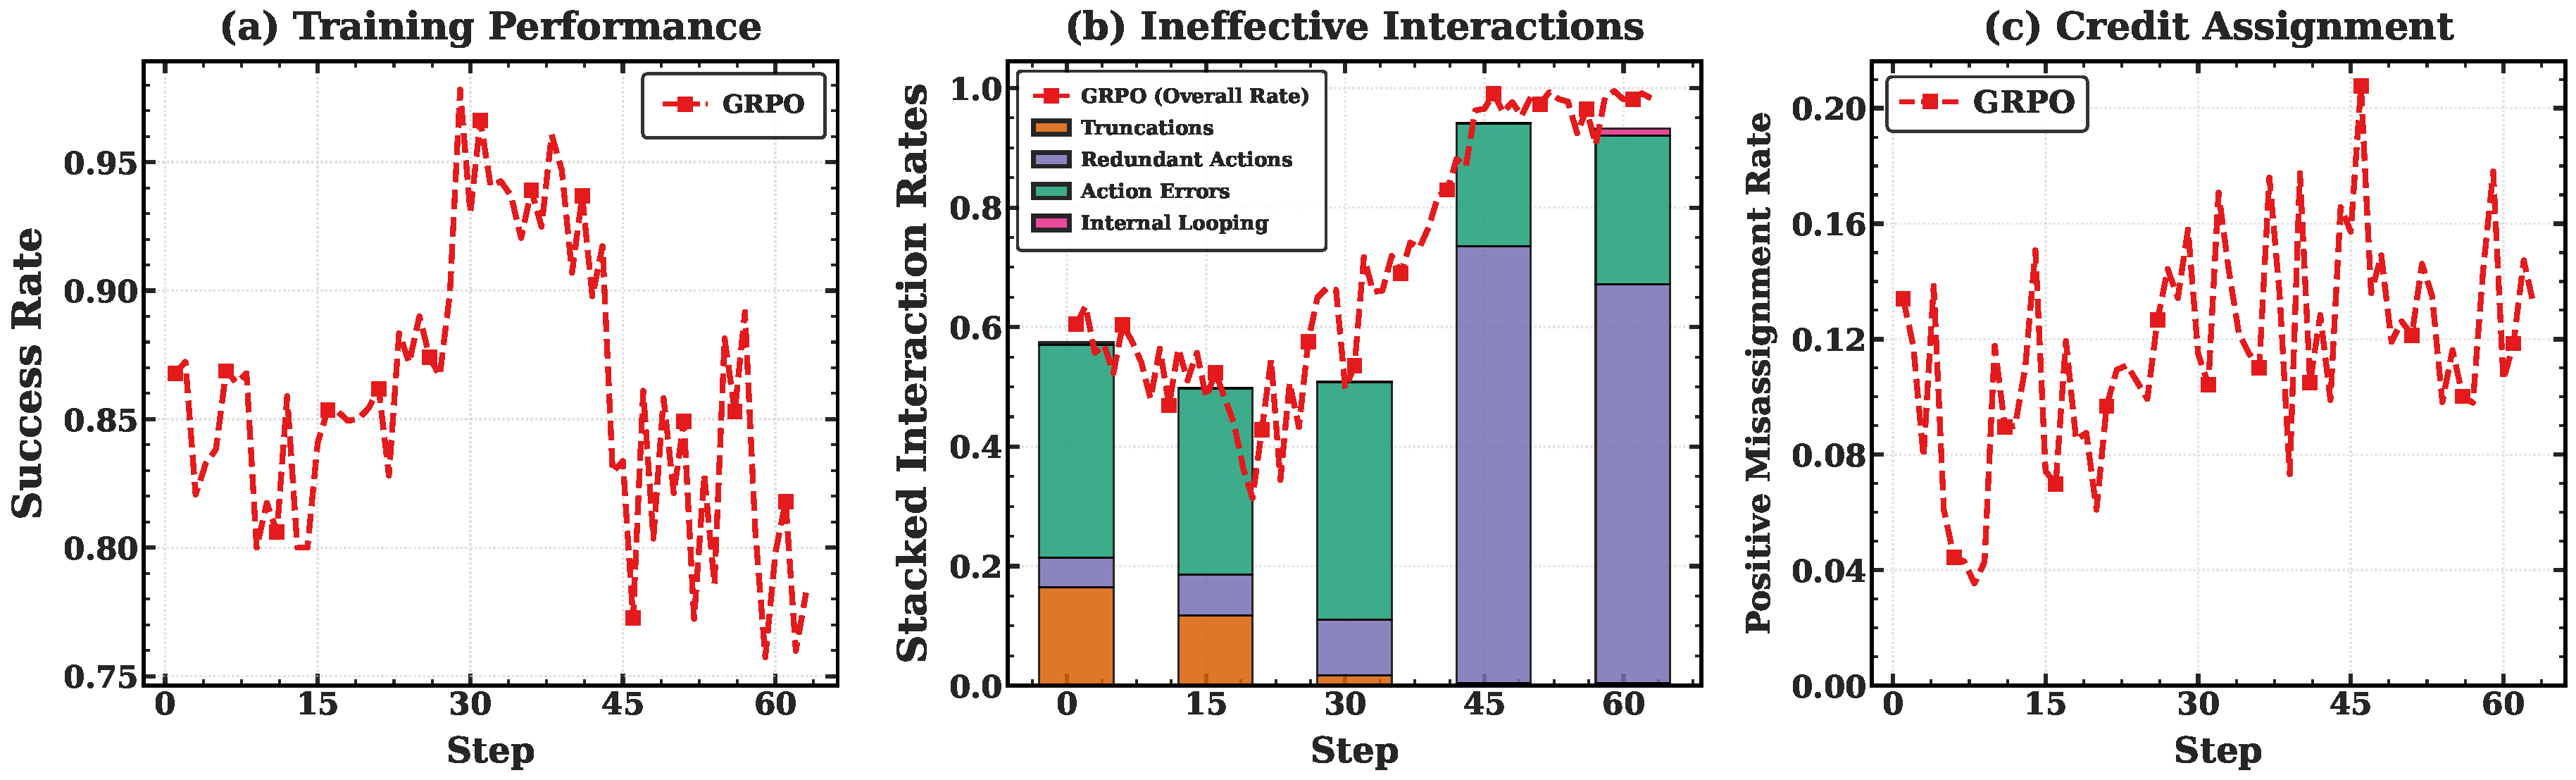
\includegraphics[width=0.8\textwidth]{./grpo_three_figures_combined.pdf}
    \caption{
    Training dynamics of GRPO vs.\ AAM on Qwen3.5-9B.
    (a) Success rate $\bar p(t)$ for GRPO;
    (b) Stacked ineffective-interaction rates $r_{\mathrm{inv}}(t)$; 
    % decomposed into internal looping, redundant actions, truncations, and action errors.
    (c) Positive-gradient misassignment $\psi_+(t)$.
    % AAM suppresses the post-peak rise of ineffective interactions and keeps positive reinforcement concentrated on productive tokens.
    % Shaded bands denote 95\% bootstrap confidence intervals.
    }
  \label{fig:intro}
\end{figure*}

\subsection{The Cost of In-Harness Rollouts}
\label{subsec:prelim_cost}
To isolate the overhead of in-harness training, we conduct a controlled comparison on a single harness, OpenClaw~\citep{openclaw}, using the DAPO-Math-17k mathematical reasoning dataset~\citep{feng2025retool}. 
We train the same model with identical generation and optimization settings under two modes:
(1) \emph{in-harness}, where rollouts execute inside the full harness (e.g., sandboxed runtime, multi-tool orchestration, observability, and session state), following \citet{bai2026clawgym}, and 
(2) \emph{tool-only}, where the LLM is augmented with a single Python-interpreter tool and no full harness environment. 
Both modes execute tools in real runtime environments and differ exclusively in their execution infrastructure.

We conduct RL training on the Qwen3-8B model using 64 GPUs.
Accounting per episode (with the per-step optimization time amortized over the global batch), the wall-clock time decomposes as:
\begin{equation}
\label{eq:wallclock}
    T_{ep} = T_{gen} + T_{env} + T_{train},
\end{equation}
where $T_{gen}$ and $T_{env}$ denote the time spent on rollout generation and environment execution/feedback, respectively, and $T_{train}$ represents the parameter optimization time.

As Fig.~\ref{fig:cost}(a) shows, environment execution accounts for {94\%} of per-episode time under in-harness training ($T_{env}=54.1$\,s), rendering it \textbf{$9.7\times$} slower than the tool-only mode on the \emph{same} task ($T_{env}=2.5$\,s). 
Crucially, this gap is not explained by tool execution alone, the tool-only mode also runs the interpreter, but by the full harness stack that surrounds it. 
Furthermore, this bottleneck is not GPU-bound: GPU utilization drastically drops from \textbf{61\%} (tool-only) to \textbf{14\%} (in-harness) (Fig.~\ref{fig:cost}(b)).
This collapse occurs because generation is brief and batched, leaving GPUs idle while the system waits on the CPU/IO-bound environment interactions following each observation. 
% synchronously waits for the CPU/IO-bound environment interactions to complete after each observation. 
% Consequently, The bottleneck is thus the environment, not the accelerator, and cannot be removed by adding GPUs.
Thus, the bottleneck is the environment, not the accelerator, and cannot be removed by adding GPUs.

\paragraph{Implication.} 
Each rollout is both computationally costly and irreplaceable for sample efficiency. 
This motivates us to build a lightweight harness that strips away non-essential harness stack components from the agent loop, thereby reducing the time overhead of environment interactions.
% during in-harness rollouts.


\begin{figure}[th]
  \centering
  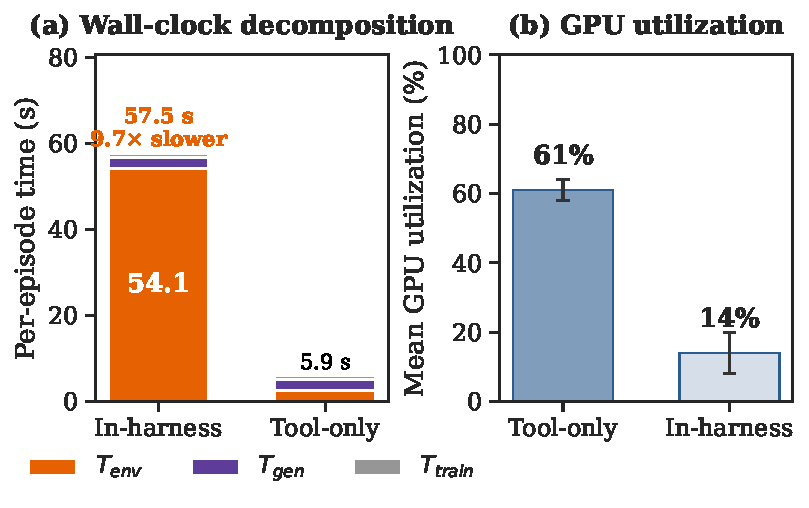
\includegraphics[width=0.4\textwidth]{./fig_cost.pdf}
  \caption{In-harness rollouts are dominated by environment execution.
  (a) Per-episode wall-clock decomposition: $T_{env}$ accounts for 94\% under in-harness training.
  % but vanishes under tool-only, yielding a $9.7\times$ slowdown. 
  (b) GPU utilization collapses from 61\% (tool-only) to 14\% (in-harness).
  % confirming a CPU/IO-bound bottleneck rather than an accelerator one.
  }
  \label{fig:cost}
\end{figure}


% \subsection{Credit Misassignment in Sparse-Reward Trajectories}
% \label{sec:motivation}
% In long-horizon tasks, the sparse nature of $R(\tau)$ creates a severe credit assignment problem. A trajectory $\tau$ may successfully complete the task (yielding $R(\tau) > 0$ and thus $\hat{A}_t > 0$ for most tokens), yet contain localized \textit{ineffective interactions}---such as infinite reasoning loops, redundant tool calls, or truncated outputs due to token budget exhaustion. 
\subsection{Train Collapse in Long-Horizon Tasks}
\label{subsec:prelim_misassign}

\paragraph{Collapse.} 
We first train Qwen3.5-9B \citep{qwen3.5} on our lightweight harness with standard GRPO and track the success rate $\bar p(t)$ (Fig.~\ref{fig:intro}a). 
% It rises to a peak $p^\star\!\approx\!0.62$ at step $t^\star$ and then \emph{collapses}: 
The curve first climbs to a peak $p^\star\!\approx\!0.95$ at step $t^\star\approx30$ and then turns downward---we call this downturn a \emph{collapse}.
we mark collapse at the first step $t_c>t^\star$ where $\bar p(t)\le p^\star$ holds for $3$ consecutive evaluations.
The verifier reward stays well-defined throughout, so the failure lies not in the objective but in how credit is assigned across a long rollout.
Under GRPO this credit is spread evenly over every token, so we argue that when a long episode succeeds by luck, its ineffective steps are reinforced together with the useful ones.
% ---precisely the misassignment we quantify next.
% confirming this reinforcement requires an intervention we defer to the ablation (\S\ref{sec:ablation})

\paragraph{Cause Analysis.}
To explain the post-$t_c$ degradation, we qualitatively inspect the failing trajectories in $[t_c, t_{\text{end}}]$ and find that their wasted effort concentrates in four recurring patterns:
% (illustrative traces in Tab.~\ref{tab:badcases}):
\begin{enumerate}[nosep,leftmargin=*]
    \item \emph{Internal Looping}---a span of tokens repeats verbatim within a turn;
    \item \emph{Redundant Actions}---an action--observation pair repeats an earlier one, yielding no new state;
    \item \emph{Truncations}---a turn is cut off at $T_{\max}$ before a valid action completes;
    \item \emph{Action Errors}---a tool call returns a failure signal ($o_n=\texttt{ERROR}$).
\end{enumerate}
% 四种trace 分别的占比，柱状图？

These four categories are \emph{induced} from the bad cases.
They are not incidental: their per-step occurrence rate $r_{\text{inv}}(t)$ tracks the collapse in anti-phase (Fig.~\ref{fig:intro}b), with a strong negative correlation (e.g., Pearson $\rho(\bar p, r_{\text{inv}})= -0.83$ and Spearman rank correlation $\rho_S\!=\!-0.90$). 
The stacked decomposition shows the post-$t_c$ surge is driven mainly by error and redundant calls, i.e.\ the very patterns that waste turns without advancing the task. 
This establishes, at the \emph{behavioral} level, that collapse co-occurs with a rising of ineffective interactions.

\begin{figure*}[t]
    \centering
    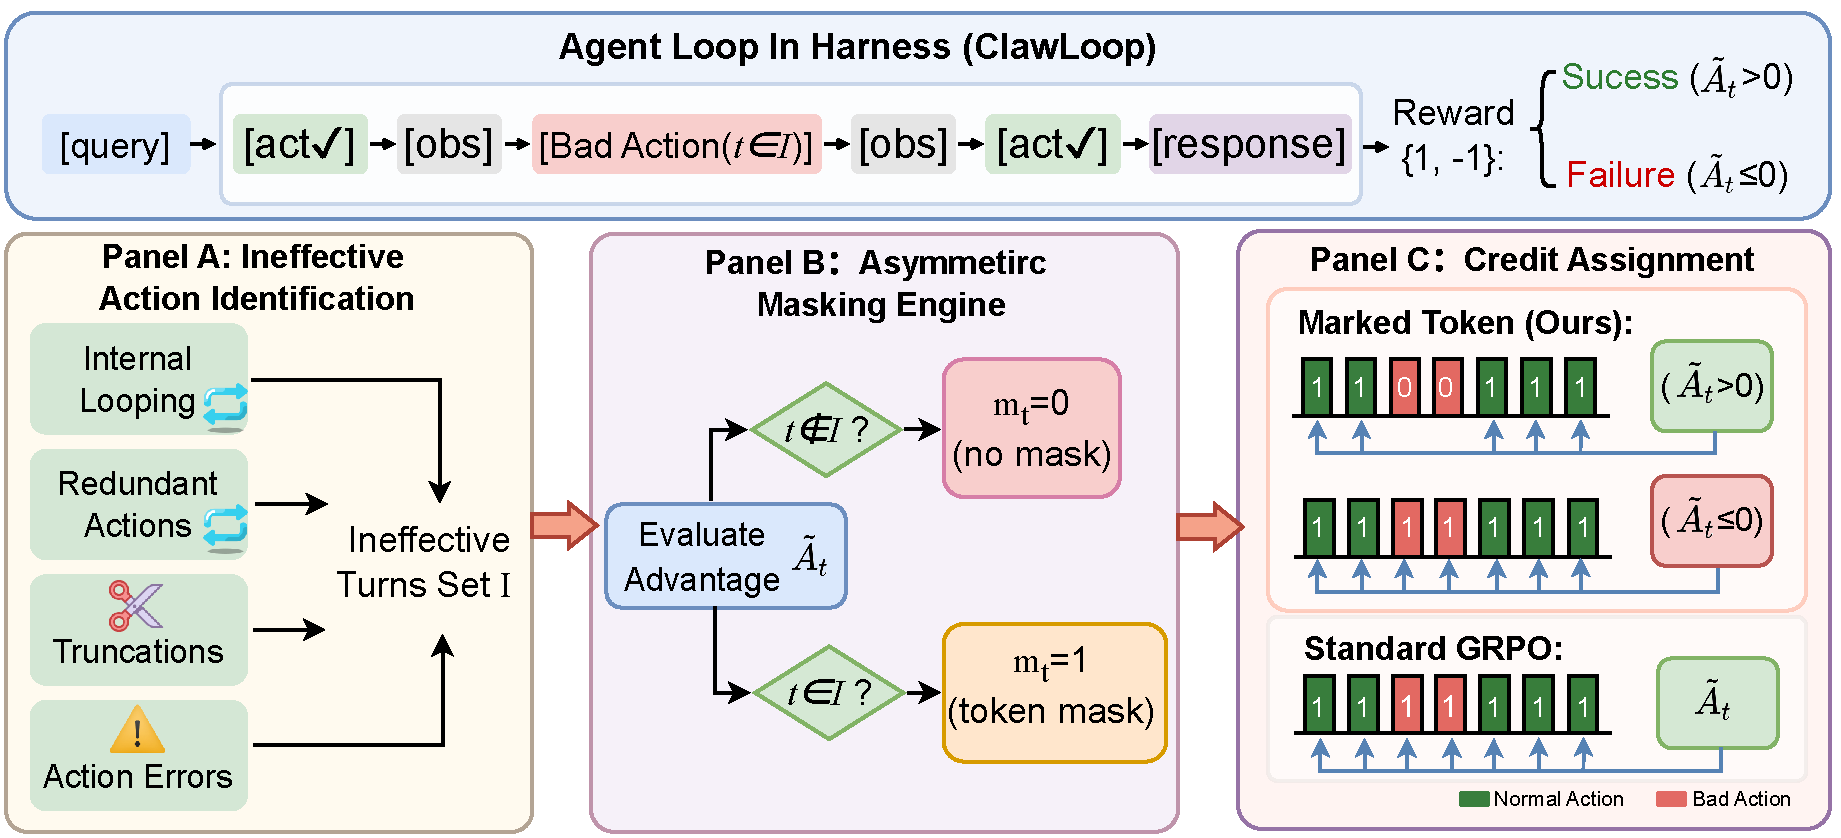
\includegraphics[width=0.8\linewidth]{clawAgent_main.pdf}
    \caption{ClawLoop-based Asymmetric Advantage Masking for RL in-Harness. 
    % The framework consists of two key components: (a) ClawLoop, a lightweight harness that minimizes environment overhead for efficient RL rollouts; and (b) 
    Asymmetric Advantage Masking (AAM) corrects credit misassignment by selectively suppressing positive gradients on ineffective tokens while preserving negative signals.}
    \label{fig:method}
\end{figure*}

% \paragraph{Gradient-Level Misassignment.}
\paragraph{Credit Misassignment.} 
However, the behavioral correlation above does not yet explain \emph{why} ineffective interactions grow. 
We therefore inspect the policy-gradient signal itself.
For a generated token $i$ in the rollouts used at training step $t$, 
let $w_i^+ = \mathbb{I}(\hat A_t>0)$ denote the positive reinforcement weight assigned by GRPO; 
the share of such mass falling on ineffective tokens is
\begin{equation}
\label{eq:psi_plus}
    \psi_+(t)
    =
    \frac{\sum_{i} w_i^+\,\mathbb{I}(i\in\mathcal{I})}
         {\sum_{i} w_i^+},
\end{equation}
where $\mathcal{I}$ be the set of tokens within ineffective interactions.
% $\psi_+$ stays low early ($\approx\!0.11$) but \emph{surges} after $t^\star$ to $\approx\!0.53$ (Fig.~\ref{fig:collapse}c): in late training, roughly half of all positive gradient lands on tokens that produced ineffective interactions. 
As shown in Fig.~\ref{fig:intro}c, $\psi_+(t)$ remains low in early training ($\approx\!0.10$) but rises sharply after the performance peak $t^\star$, reaching $\approx\!0.21$ in the collapse region.
% Thus, by late training, roughly half of the positive learning signal is assigned to tokens that participate in ineffective interactions.
% Because GRPO broadcasts the trajectory-level advantage to every token, the ineffective tokens of a successful episode are reinforced alongside the effective ones.
% Therefore, we summarize that 
% % This provides a gradient-level explanation for the behavioral trend observed above: 
% collapse is not merely accompanied by ineffective interactions; it is actively amplified by credit misassignment, confirming that successful trajectories themselves grow hollow.
As shown in Fig.~\ref{fig:intro}c, $\psi_+(t)$ rapidly decreases from $0.12$ to $0.04$ within the first 10 steps. However, during steps 15--30, it surges quickly to $0.16$ and reaches a peak of $0.20$---precisely aligning with the rapid drop in success rate in Fig.~\ref{fig:intro}a.
Thus, in this region, a significant portion of the positive learning signal is misassigned to tokens that participate in ineffective interactions.
Because GRPO broadcasts the trajectory-level advantage to every token, the ineffective tokens of a successful episode are reinforced alongside the effective ones.
Therefore, we summarize that collapse is not merely accompanied by ineffective interactions; it is actively amplified by credit misassignment, confirming that successful trajectories themselves grow hollow.
% Because GRPO broadcasts the trajectory-level advantage uniformly over all generated tokens, a successful but inefficient episode reinforces its wasted steps together with its productive ones.


\paragraph{Implication.}
% These results suggest that 
Credit misassignment contributes to training collapse.
To align the optimization signal with the actual contribution of each token, we propose the asymmetric advantage masking strategy introduced next.

% todo 
% 2，添加图片设计说明mask+harness，
% while preserving their negative gradient signals.
% for RL in long-horizon agents training. 
% formalize the credit misassignment problem inherent in standard Reinforcement Learning (RL) for long-horizon agents and 
% To rectify this fine-grained credit misassignment, 
% Instead of discarding the entire trajectory or altering the verifier reward
\section{Methodology}
In this section, we present our framework for efficient and robust agent RL.
We propose \emph{ClawLoop}, a lightweight harness that minimizes environment overhead, and \emph{Asymmetric Advantage Masking}, which corrects credit misassignment by suppressing spurious positive gradients (Fig.~\ref{fig:method}).
% We first introduce \textbf{ClawLoop}, a lightweight harness that strips away product-level overhead to accelerate in-harness rollouts (\S\ref{subsec:nanoclaw}).
% Building on this efficient infrastructure, we propose \emph{Asymmetric Advantage Masking} (AAM), a token-level correction mechanism that selectively suppresses spurious positive gradients on ineffective actions while preserving negative signals, thereby resolving the credit misassignment problem identified in \S\ref{sec:prelim} (\S\ref{subsec:aam}).

% 基本设计思路
% 具体如何设计的？减少了什么？如何减少的？
% 效果如何，量化分析？实验中操作?
% 嵌入 RL 训练闭环
\subsection{ClawLoop: A Lightweight Harness}
\label{subsec:nanoclaw}

\paragraph{From Product to Training.}
Product agent harness are typically optimized for user-facing functionality rather than gradient estimation.
Starting from OpenClaw~\citep{openclaw}, a product-oriented, open-source agent harness, we reconstruct a white-box, lightweight training harness, {ClawLoop}.
Unlike black-box harnesses that expose only final textual outputs, ClawLoop exposes a unified rollout record of environment state (workspace file snapshots and tool execution logs), interaction history (per-step prompts and generated responses), and token-level log-probabilities of generated tokens.
This design enables the RL system to compute policy gradients directly from the rollout, without parsing or reverse-engineering external product APIs.

ClawLoop follows a single design principle: \emph{remove product-level complexity while retaining the minimal interaction loop required for agent RL.}
Concretely, we remove the following components from the rollout critical path: persistent sessions and cross-episode state, long-term memory and user profiles, dynamic plugin registries and third-party service connections, background tasks and multi-agent orchestration, and authentication and permission control.
These modules are essential for real-world deployment, but in RL rollouts they introduce hidden-state variance, uncontrollable external failure modes, and dynamically changing action spaces.
The retained core is a minimal five-component closed loop comprising task specification, environment state, tool execution, multi-turn interaction, and terminal verification.
Fig.~\ref{fig:method} illustrates the resulting architecture and its data flow within the RL system.

\paragraph{Integration with RL training.}
ClawLoop is integrated as a thin environment interface into the \textsc{verl} distributed RL system~\citep{sheng2024verl}, leaving the sampling scheduler and parameter-update logic unchanged.
Each episode constitutes a finite-horizon MDP: the state $s_t=(q,\,o_{\leq t})$ concatenates the task instruction with observation history; transitions are deterministic given tool execution; reward is provided only at the terminal step by the verifier.
This clean separation follows directly from the simplification above: with no shared memory, background services, or cross-episode dependencies, $N$ trajectories can be executed independently on $N$ workers. 
Each worker maintains a single lightweight sandbox process, so tool errors in one trajectory do not contaminate others.
As a result, per-episode environment-side overhead is reduced from $54.1\,\mathrm{s}$ (\S\ref{subsec:prelim_cost}) to ${\sim}5$\,s (detailed in \S\ref{sec:experiments}), and system throughput is primarily bounded by model inference throughput.
% A complete episode trace under the real training protocol is provided in Appendix~\ref{app:episode}.


\subsection{Asymmetric Advantage Masking}
\paragraph{Ineffective Interaction Identification}
We instantiate the four patterns from \S\ref{sec:prelim} as deterministic, environment-side rules over the rollout. Let $\mathcal{T}_n$ be the indices of the tokens \emph{generated} by the $n$-th assistant turn; prompt, observation, and padding tokens are excluded from all rules and from the loss. The union of flagged indices defines the global ineffective set $\mathcal{I}\subset\{1,\dots,T\}$:
\begin{enumerate}
    \item \textbf{Internal Looping.} A repeated span $x_{t:t+k-1}=x_{t+k:t+2k-1}$ with $k\ge k_{\min}$ flags its redundant copy $\{t+k,\dots,t+2k-1\}$.
    \item \textbf{Redundant Actions.} A turn $n$ with $(a_n,o_n)=(a_{n'},o_{n'})$ for some $n'<n$ flags $\mathcal{T}_n$.
    \item \textbf{Truncations.} A turn cut off at the response budget $T_{\max}$ flags $\mathcal{T}_n$.
    \item \textbf{Action Errors.} A turn whose observation is a failure signal ($o_n=\texttt{ERROR}$) flags $\mathcal{T}_n$.
\end{enumerate}


\paragraph{Asymmetric Token-Level Masking}
Let $m_t^{\text{base}} \in \{0, 1\}$ be the standard masking vector (e.g., masking out padding tokens or prompt tokens). We introduce the asymmetric masking vector $m_t \in \{0, 1\}$, defined as:
\begin{equation}
\label{eq:asymmetric_mask}
    m_t = m_t^{\text{base}} \cdot \left[ 1 - \mathbb{I}\left( t \in \mathcal{I} \land \hat{A}_t > 0 \right) \right],
\end{equation}
where $\mathbb{I}(\cdot)$ is the indicator function. 
The indicator fires only when an ineffective token carries a \emph{positive} advantage. 
In GRPO the advantage is trajectory-level, $\hat{A}_t\equiv\hat{A}(\tau)$, so this is exactly the case where the episode was rewarded.

% \textbf{Motivation for Asymmetry:} The core design principle lies in the condition $\hat{A}_t > 0$. 
% \begin{itemize}
%     \item \textit{When $\hat{A}_t > 0$ (Positive Advantage):} If $t \in \mathcal{I}$, the mask $m_t$ is set to 0. This blocks the erroneous positive reinforcement, preventing the policy from increasing the probability of ineffective interactions simply because the overall trajectory succeeded.
%     \item \textit{When $\hat{A}_t \le 0$ (Negative Advantage):} Even if $t \in \mathcal{I}$, the indicator evaluates to 0, keeping $m_t = m_t^{\text{base}}$. This ensures that the negative gradient signal is preserved. The model is still penalized for generating these ineffective interactions in failed trajectories, allowing it to learn the correct negative association.
% \end{itemize}
% This asymmetric design ensures that we only \textit{ignore} the ineffective interaction when the environment accidentally rewards it, but we actively \textit{punish} it when the environment penalizes it, maintaining a complete and directional learning signal.

This asymmetric design ensures that we only \textit{ignore} ineffective interactions when accidentally rewarded, but actively \textit{punish} them when penalized, maintaining a complete and directional learning signal.

\paragraph{Policy Optimization with Masked Objectives}
We integrate the asymmetric mask $m_t$ into the GRPO objective to form the Masked GRPO loss. 
The updated actor objective is computed as:
\begin{equation}
\label{eq:masked_grpo}
    \begin{aligned}
        \mathcal{J}_{\text{Masked}}(\theta) &= \mathbb{E}_{\tau}\!\left[ \frac{1}{\sum_{t=1}^{T} m_t} \sum_{t=1}^{T} m_t \, \ell_t(\theta) \right], \\
        \ell_t(\theta) &= \min\!\Big( \rho_t \hat{A}_t,\; \operatorname{clip}\!\big(\rho_t,\, 1{-}\epsilon,\, 1{+}\epsilon\big)\, \hat{A}_t \Big),
    \end{aligned}
\end{equation}
By re-weighting the loss with $m_t$, the optimization process dynamically excludes the tokens of ineffective interactions in successful trajectories from the policy gradient update. 
% todo 添加reward 设计,

% Crucially, this mechanism operates entirely at the token level without modifying the underlying agent loop, altering the verifier rewards, or truncating the context required for subsequent autoregressive generation.
Overall, this method acts as a fine-grained credit assignment corrector, effectively decoupling local behavioral quality from global trajectory outcomes in long-horizon agent training.
% Normalizing by the effective count $\sum_t m_t$ (rather than $T$) prevents masked tokens from diluting the length-normalized update. 
% AAM is purely a post-hoc loss re-weighting: it leaves the agent loop, verifier, and autoregressive context untouched, acting as a fine-grained credit-assignment corrector for long-horizon training.

\section{Experiments}
\label{sec:experiments}

\subsection{Setup}
\paragraph{Training data.}
Since no off-the-shelf corpus exists for claw-style agent training, we construct one by adapting the task-synthesis pipeline of ClawBenchPro~\citep{clawbenchpro}. 
The resulting dataset contains $7{,}000$ instances, each defined as a triple $(q, \mathcal{W}_0, \mathcal{V})$: a natural-language task $q$, an initial workspace snapshot $\mathcal{W}_0$, and a deterministic terminal-state verifier $\mathcal{V}$.
During rollout, the agent receives $q$ and $\mathcal{W}_0$ as initial context; $\mathcal{V}$ is queried only at episode end to produce $R(\tau)\in\{-1,1\}$.
% Crucially, the synthesizer produces only verifiable task specifications rather than expert trajectories.


\paragraph{Evaluation.} 
We evaluate on two groups of benchmarks:
% We evaluate on two groups of benchmarks to assess both in-distribution performance and generalization.
The \emph{in-domain} group comprises three claw-style agent benchmarks: 
PinchBench~\citep{kiloaiteam2026pinchbench}, ClawEval~\citep{ye2026claw}, and ClawBenchPro~\citep{clawbenchpro}, which share the workspace-and-tool interaction format of training.
% todo, 一句话，介绍数据集ClawBenchPro
The \emph{out-of-domain} group comprises two widely used multi-turn tool-use benchmarks, BFCL-v3~\citep{patil2025bfcl} and $\tau^2$-bench~\citep{barres2025tau2}, whose tool schemas and dialogue protocols differ from training; strong performance here indicates that the learned agent behavior transfers beyond the synthetic distribution.
For all benchmarks, we run three times and report both the average success rate.
% The \emph{in-domain} group comprises three claw-style agent benchmarks---PinchBench~\citep{kiloaiteam2026pinchbench}, ClawEval~\citep{claweval}, and ClawBenchPro~\citep{nanoclaw2026}---which share the same workspace-and-tool interaction format as our training data.
% The \emph{out-of-domain} group includes two widely used multi-turn tool-use benchmarks, BFCL-v3~\citep{patil2025bfcl} and $\tau^2$-bench~\citep{barres2025tau2}. 
% These benchmarks feature distinct tool schemas and dialogue protocols, serving as a rigorous test of whether the learned agent behavior transfers beyond the synthetic training distribution.

% \begin{table*}[th]
%     \centering
%     \small
%     \begin{tabular}{l cc cc cc}
%         \toprule
%         & \multicolumn{2}{c}{PinchBench} & \multicolumn{2}{c}{ClawEval} & \multicolumn{2}{c}{ClawBenchPro} \\
%         \cmidrule(lr){2-3} \cmidrule(lr){4-5} \cmidrule(lr){6-7}
%         Method & SR & P@3 & SR & P@3 & SR & P@3 \\
%         \midrule
%         \multicolumn{7}{l}{\textit{Proprietary}} \\
%         GPT-5            & -- & -- & -- & -- & -- & -- \\
%         Claude 4.6       & -- & -- & -- & -- & -- & -- \\
%         DeepSeek-V4      & -- & -- & -- & -- & -- & -- \\
%         \midrule
%         \multicolumn{7}{l}{\textit{Open-source (Qwen3.5-9B)}} \\
%         \rowcolor{gray!10} Base     & 49.40 & 29.41 & 65.20 & 65.60 & 88.00 & 72.20 \\
%         \hspace{2pt} + GRPO           & 52.10 & 32.91 & 67.50 & 67.50 & 90.10 & 73.60 \\
%         \hspace{2pt} + AAM (ours)     & 57.20 & 39.50 & 71.60 & 71.09 & 93.60 & 76.30 \\
%         \midrule
%         \multicolumn{7}{l}{\textit{Scale comparison (AAM)}} \\
%         \rowcolor{gray!10} Qwen3.5-2B       & 26.80 & 13.45 & 29.10 & 28.90 & 63.70 & 26.50 \\
%         \hspace{2pt} + AAM     & 41.80 & 20.17 & 50.40 & 40.60 & 73.70 & 32.70 \\
%         \rowcolor{gray!10} Qwen3.5-4B       & 37.10 & 23.53 & 58.90 & 57.80 & 87.60 & 63.00 \\
%         \hspace{2pt} + AAM     & 50.80 & 35.29 & 72.40 & 68.80 & 91.10 & 68.30 \\
%         \rowcolor{gray!10} Qwen3.5-27B      & 52.04 & 33.60 & 72.30 & 72.60 & 93.70 & 81.40 \\
%         \hspace{2pt} + AAM     & 57.54 & 40.80 & 75.80 & 76.10 & 95.80 & 84.30 \\
%         \bottomrule
%     \end{tabular}
%     \caption{Results on claw-style agent benchmarks. All models evaluated under OpenClaw. Best open-source in \textbf{bold}, best overall \underline{underlined}.
%     % todo add result analysis 
%     }
%     \label{tab:main_claw}
% \end{table*}

% \begin{table}[th]
%     \centering
%     \small
%     \begin{tabular}{l c c c}
%         \toprule
%         Method & PinchBench & ClawEval & ClawBenchPro \\
%         \midrule
%         \multicolumn{4}{l}{\textit{Proprietary}} \\
%         Kimi-2.5          & 54.60 & 66.60 & 73.00 \\
%         Claude-4.6-Opus   & 69.90 & 80.60 & 92.30 \\
%         GPT-5.4           & 75.70 & 78.30 & 93.70 \\
%         MiniMax-m2.7      & 65.40 & 71.80 & 78.20 \\
%         Nemotron3Super    & 42.20 & 41.70 & 46.50 \\
%         \midrule
%         \multicolumn{4}{l}{\textit{Open-source (Qwen3.5-9B)}} \\
%         \rowcolor{gray!10} Base     & 49.40 & 65.20 & 88.00 \\
%         \hspace{2pt} + GRPO         & 52.10 & 67.50 & 90.10 \\
%         \hspace{2pt} + AAM (ours)   & 57.20 & 71.60 & 93.60 \\
%         \midrule
%         \multicolumn{4}{l}{\textit{Scale comparison (AAM)}} \\
%         \rowcolor{gray!10} Qwen3.5-2B     & 26.80 & 29.10 & 63.70 \\
%         \hspace{2pt} + AAM           & 41.80 & 50.40 & 73.70 \\
%         \rowcolor{gray!10} Qwen3.5-4B     & 37.10 & 58.90 & 87.60 \\
%         \hspace{2pt} + AAM           & 50.80 & 72.40 & 91.10 \\
%         \rowcolor{gray!10} Qwen3.5-27B    & 52.04 & 72.30 & 93.70 \\
%         \hspace{2pt} + AAM           & 57.54 & 75.80 & 95.80 \\
%         \bottomrule
%     \end{tabular}
%     \caption{Results on claw-style agent benchmarks. All models evaluated under OpenClaw. Best open-source in \textbf{bold}, best overall \underline{underlined}.
%     % todo add result analysis 
%     }
%     \label{tab:main_claw}
% \end{table}



\providecommand{\err}[1]{{\scriptsize\color{gray}$\pm$#1}}

\begin{table}[th]
    \centering
    \small
    \begin{tabular}{l c c c}
        \toprule
        Method & PinchBench & ClawEval & ClawBenchPro \\
        \midrule
        \multicolumn{4}{l}{\textit{Proprietary}} \\
        Kimi-2.5          & 54.60 & 66.60 & 73.00 \\
        Claude-4.6-Opus   & 69.90 & 80.60 & 92.30 \\
        GPT-5.4           & 75.70 & 78.30 & 93.70 \\
        MiniMax-m2.7      & 65.40 & 71.80 & 78.20 \\
        Nemotron3Super    & 42.20 & 41.70 & 46.50 \\
        \midrule
        \multicolumn{4}{l}{\textit{Open-source (Qwen3.5-9B)}} \\
        \rowcolor{gray!10} Base     & 49.40\err{0.4} & 65.20\err{0.3} & 88.00\err{0.2} \\
        \hspace{2pt} + GRPO         & 52.10\err{0.3} & 67.50\err{0.5} & 90.10\err{0.2} \\
        \hspace{2pt} + AAM (ours)   & 57.20\err{0.2} & 71.60\err{0.4} & 93.60\err{0.1} \\
        \midrule
        \multicolumn{4}{l}{\textit{Scale comparison (AAM)}} \\
        \rowcolor{gray!10} Qwen3.5-2B     & 26.80\err{0.5} & 29.10\err{0.6} & 63.70\err{0.4} \\
        \hspace{2pt} + AAM               & 41.80\err{0.3} & 50.40\err{0.4} & 73.70\err{0.3} \\
        \rowcolor{gray!10} Qwen3.5-4B     & 37.10\err{0.4} & 58.90\err{0.3} & 87.60\err{0.3} \\
        \hspace{2pt} + AAM               & 50.80\err{0.2} & 72.40\err{0.3} & 91.10\err{0.2} \\
        \rowcolor{gray!10} Qwen3.5-27B    & 52.04\err{0.3} & 72.30\err{0.2} & 93.60\err{0.1} \\
        \hspace{2pt} + AAM               & 57.54\err{0.2} & 75.80\err{0.3} & 95.80\err{0.1} \\
        \bottomrule
    \end{tabular}
    \caption{Results on claw-style agent benchmarks. Reported values are mean $\pm$ std across 3 random seeds.}
    \label{tab:main_claw}
\end{table}


% \paragraph{Implementation and Baselines.}
% We fine-tune Qwen3.5 models from 2B to 27B parameters with RL, selecting this series because it already exhibits basic proficiency in harness.
% We use GRPO within the VERL framework~\citep{sheng2024verl}, with ClawLoop as the interaction harness.
% Training is conducted on 40 GPUs with a rollout batch size of 64, update mini-batch size of 8, a 32K token context window, and up to 64 action turns per trajectory;
% full details are in SM.
% % Appendix~\ref{app:impl_details}. 
% We compare against open-source Qwen3.5 baselines and top-tier proprietary models (GPT-5~\citep{OpenAIGPT5}, Claude 4.6~\citep{anthropic2024claude46}), 
% all evaluated under the standard OpenClaw harness to ensure fair comparison on complex multi-turn tasks.
% At inference time, enable thinking mode; leave other parameters at their defaults.
\paragraph{Implementation and Baselines.}
We fine-tune Qwen3.5 models (2B–27B) with RL, selecting this series as it has basic harness proficiency.
We use GRPO within the VERL framework~\citep{sheng2024verl}, with ClawLoop as the interaction harness.
Training is conducted on 40 GPUs with a rollout batch size of 64, update mini-batch size of 8, a 32K token context window, and up to 64 action turns per trajectory (details in SM).
We compare against open-source Qwen3.5 baselines and top-tier proprietary models (GPT-5~\citep{OpenAIGPT5}, Claude 4.6~\citep{anthropic2024claude46}), 
all evaluated under the standard OpenClaw harness for fair comparison on complex multi-turn tasks.
At inference, we enable thinking mode and keep other parameters as defaults.
% During the inference phase, enable the thinking mode and keep all other model parameters at their default settings.
% same NanoClaw-RL
% 其他的值得说的超参数说明 ？

\subsection{Main Results}
\label{subsec:main_results}
% 两段，P1 claw benchmark 分析， P2 tool-use benchmark 分析。
% Tables~\ref{tab:main_claw} and~\ref{tab:main_tool} report success rate (SR) and Pass@3 on claw-style and tool-use benchmarks, respectively.
% On three claw-style benchmarks (Tables~\ref{tab:main_claw}), AAM consistently outperforms standard GRPO across every model scale.
% The gain is largest on \textsc{ClawBenchPro} ($+\textbf{X.X}$ SR on Qwen3.5-9B), followed by \textsc{ClawEval} ($+\textbf{X.X}$) and \textsc{PinchBench} ($+\textbf{X.X}$).
% This ordering aligns with task horizon: \textsc{ClawBenchPro} contains the longest and most compositional episodes, where credit misassignment is most severe and suppressing reinforcement of ineffective tokens yields the largest return.
% Pass@3 improves in parallel with SR, indicating that AAM increases not only average competence but also cross-run reliability.
% Moreover, its success rate is comparable to that of frontier API-based LLMs with over 300B parameters.
% At 27B scale, AAM reaches \textbf{XX.X}\% SR, narrowing the gap to GPT-5 (\textbf{XX.X}\%) from \textbf{X.X} to \textbf{X.X} points, suggesting that better credit assignment can partially substitute for scale.
% On the two tool-use benchmarks (Tables~\ref{tab:main_tool}), AAM also transfers out-of-domain: 
% it improves over GRPO by $+\textbf{X.X}$ on BFCL-v3 and $+\textbf{X.X}$ on $\tau^2$-bench (Table~\ref{tab:main_tool}), despite these benchmarks using different tool schemas and dialogue protocols.
% This transfer is notable because the training data contains no BFCL or $\tau^2$-bench tasks; the gain therefore reflects a general improvement in multi-turn planning and error recovery rather than format memorization.
% We attribute this to AAM concentrating gradient on informative actions, which produces cleaner tool-call sequences that generalize across schemas.
% Consistent with this explanation, the gain is largest on the longer $\tau^2$-bench domains (Airline and Telecom), mirroring the trend observed on claw-style benchmarks.
% Overall, these results indicate that correcting credit misassignment benefits not only in-distribution task completion but also cross-domain tool use.
On three claw-style benchmarks (Table~\ref{tab:main_claw}), AAM consistently outperforms standard GRPO across every model scale.
The gain is largest on \textsc{PinchBench} ($+\textbf{5.10}$ SR on Qwen3.5-9B), followed by \textsc{ClawEval} ($+\textbf{4.10}$) and \textsc{ClawBenchPro} ($+\textbf{3.60}$).
This ordering aligns with task horizon: \textsc{PinchBench} contains the longest and most compositional episodes, where credit misassignment is most severe and suppressing reinforcement of ineffective tokens yields the largest return.
% Pass@3 improves in parallel with SR, indicating that AAM increases not only average competence but also cross-run reliability.
Moreover, its success rate is comparable to that of frontier API-based LLMs with over 300B parameters.
At 27B scale, AAM reaches \textbf{95.80}\% SR on ClawBenchPro, narrowing the gap to GPT-5.4 (\textbf{93.70}\%) from a \textbf{0.10} point difference to outperforming it by \textbf{2.10} points, suggesting that better credit assignment can partially substitute for scale.

On two tool-use benchmarks (Tables~\ref{tab:main_tool}), AAM also transfers out-of-domain: 
% it improves over GRPO by $+\textbf{3.15}$ on BFCL-v3 and $+\textbf{3.33}$ on $\tau^2$-bench (Table~\ref{tab:main_tool}), despite these benchmarks using different tool schemas and dialogue protocols.
it improves over GRPO by $+\textbf{3.15}$ on BFCL-v3 and $+\textbf{3.33}$ on $\tau^2$-bench, despite differing tool schemas and dialogue protocols.
This transfer is notable because training data contains no BFCL or $\tau^2$-bench tasks; the gain therefore reflects a general improvement in multi-turn planning and error recovery rather than format memorization.
We attribute this to AAM concentrating gradients on informative actions, which produces cleaner tool-call sequences that generalize across schemas.
% Consistent with this explanation, the gain is largest on the longer $\tau^2$-bench domains (Airline and Telecom), mirroring the trend observed on claw-style benchmarks.
Accordingly, the gain is largest on longer $\tau^2$-bench domains (Airline and Telecom), mirroring the trend observed on claw-style benchmarks.
Overall, correcting credit misassignment benefits not only in-distribution task completion but also cross-domain tool use.


% \begin{table}[t]
%     \centering
%     \small
%     \begin{tabular}{l cc cc}
%         \toprule
%         & \multicolumn{1}{c}{BFCL-v3} & \multicolumn{3}{c}{$\tau^2$-bench} \\
%         \cmidrule(lr){2-2} \cmidrule(lr){3-5}
%         Method & Overall & Retail & Airline & Telecom \\
%         \midrule
%         \multicolumn{5}{l}{\textit{Proprietary}} \\
%         GPT-5            & -- & -- & -- & -- \\
%         Claude 4.6       & -- & -- & -- & -- \\
%         DeepSeek-V4      & -- & -- & -- & -- \\
%         \midrule
%         \multicolumn{5}{l}{\textit{Open-source (Qwen3.5-9B)}} \\
%         \rowcolor{gray!10} Base     & 44.00 & -- & -- & -- \\
%         \hspace{2pt} + GRPO           & 45.60 & -- & -- & -- \\
%         \hspace{2pt} + AAM (ours)     & 48.75 & -- & -- & -- \\
%         \midrule
%         \multicolumn{5}{l}{\textit{Scale comparison (AAM)}} \\
%         \rowcolor{gray!10} Qwen3.5-2B       & 31.50 & -- & -- & -- \\
%         \hspace{2pt} + AAM     & 40.50 & -- & -- \\
%         \rowcolor{gray!10} Qwen3.5-4B       & 44.25 & -- & -- & -- \\
%         \hspace{2pt} + AAM     & 48.5 & -- & -- \\
%         \rowcolor{gray!10} Qwen3.5-27B      & 61.0 & -- & -- & -- \\
%         \hspace{2pt} + AAM     & 64.5 & -- & -- \\
%         \bottomrule
%     \end{tabular}
%     \caption{Out-of-domain results on multi-turn tool-use benchmarks. % todo add result analysis 
%     }
%     \label{tab:main_tool}
% \end{table}

% \begin{table}[t]
%     \centering
%     \small
%     \begin{tabular}{l cc cc}
%         \toprule
%         & \multicolumn{1}{c}{BFCL-v3} & \multicolumn{3}{c}{$\tau^2$-bench} \\
%         \cmidrule(lr){2-2} \cmidrule(lr){3-5}
%         Method & Overall & Retail & Airline & Telecom \\
%         \midrule
%         \multicolumn{5}{l}{\textit{Proprietary}} \\
%         Gemini-3-Pro            & 60.75 & 75.90 & 80.50 & 91.00 \\
%         Claude Sonnet 4.5       & 61.37 & 72.40 & 72.00 & 84.90 \\
%         Qwen3-235B-Thinking      & 42.75 & 71.90 & 58.60 & 47.30 \\
%         Kimi-K2-Instruct      & 45.88 & 70.6 & 56.50 & 65.80 \\
%         \midrule
%         \multicolumn{5}{l}{\textit{Open-source (Qwen3.5-9B)}} \\
%         \rowcolor{gray!10} Base     & 44.00 & 35.14 & 32.00 & 15.79 \\
%         \hspace{2pt} + GRPO         & 45.60 & 36.18 & 34.00 & 17.93 \\
%         \hspace{2pt} + AAM (ours)   & 48.75 & 38.23 & 37.94 & 22.15 \\
%         \midrule
%         \multicolumn{5}{l}{\textit{Scale comparison (AAM)}} \\
%         \rowcolor{gray!10} Qwen3.5-2B       & 31.50 & 25.44 & 16.00 & 35.96 \\
%         \hspace{2pt} + AAM                  & 40.50 & 31.30 & 27.25 & 48.01 \\
%         \rowcolor{gray!10} Qwen3.5-4B       & 44.25 & 38.60 & 30.00 & 49.12 \\
%         \hspace{2pt} + AAM                  & 48.50 & 41.37 & 35.31 & 54.81 \\
%         \rowcolor{gray!10} Qwen3.5-27B      & 61.00 & 64.91 & 72.00 & 73.68 \\
%         \hspace{2pt} + AAM                  & 64.50 & 67.19 & 76.38 & 78.37 \\
%         \bottomrule
%     \end{tabular}
%     \caption{Out-of-domain results on multi-turn tool-use benchmarks. % todo add result analysis 
%     }
%     \label{tab:main_tool}
% \end{table}

\providecommand{\err}[1]{{\scriptsize\color{gray}$\pm$#1}}

\begin{table}[t]
    \centering
    \footnotesize
    % @{} 消除表格最左和最右的留白，精细控制列与列之间的间距为 1.5pt
    \setlength{\tabcolsep}{1.5pt} 
    \begin{tabular}{@{} l c c c c @{}}
        \toprule
        & \multicolumn{1}{c}{BFCL-v3} & \multicolumn{3}{c}{$\tau^2$-bench} \\
        \cmidrule(lr){2-2} \cmidrule(lr){3-5}
        Method & Overall & Retail & Airline & Telecom \\
        \midrule
        \multicolumn{5}{@{}l}{\textit{Proprietary}} \\
        Gemini-3-Pro            & 60.75 & 75.90 & 80.50 & 91.00 \\
        Claude Sonnet 4.5       & 61.37 & 72.40 & 72.00 & 84.90 \\
        Qwen3-235B-Think        & 42.75 & 71.90 & 58.60 & 47.30 \\
        Kimi-K2-Instruct        & 45.88 & 70.60 & 56.50 & 65.80 \\
        \midrule
        \multicolumn{5}{@{}l}{\textit{Open-source (Qwen3.5-9B)}} \\
        \rowcolor{gray!10} Base     & 44.00\err{0.4} & 35.14\err{0.3} & 32.00\err{0.5} & 15.79\err{0.2} \\
        \hspace{2pt} + GRPO         & 45.60\err{0.3} & 36.18\err{0.4} & 34.00\err{0.3} & 17.93\err{0.2} \\
        \hspace{2pt} + AAM (ours)   & 48.75\err{0.2} & 38.23\err{0.3} & 37.94\err{0.2} & 22.15\err{0.1} \\
        \midrule
        \multicolumn{5}{@{}l}{\textit{Scale comparison (AAM)}} \\
        \rowcolor{gray!10} Qwen3.5-2B       & 31.50\err{0.5} & 25.44\err{0.4} & 16.00\err{0.6} & 35.96\err{0.5} \\
        \hspace{2pt} + AAM                  & 40.50\err{0.3} & 31.30\err{0.3} & 27.25\err{0.4} & 48.01\err{0.3} \\
        \rowcolor{gray!10} Qwen3.5-4B       & 44.25\err{0.4} & 38.60\err{0.3} & 30.00\err{0.3} & 49.12\err{0.4} \\
        \hspace{2pt} + AAM                  & 48.50\err{0.2} & 41.37\err{0.2} & 35.31\err{0.2} & 54.81\err{0.2} \\
        \rowcolor{gray!10} Qwen3.5-27B      & 61.00\err{0.3} & 64.91\err{0.2} & 72.00\err{0.3} & 73.68\err{0.2} \\
        \hspace{2pt} + AAM                  & 64.50\err{0.1} & 67.19\err{0.2} & 76.38\err{0.1} & 78.37\err{0.1} \\
        \bottomrule
    \end{tabular}
    % \caption{Out-of-domain results on multi-turn tool-use benchmarks. Values are reported as mean $\pm$ std across 3 random seeds.}
    \caption{Out-of-domain results on multi-turn tool-use benchmarks. Reported as mean $\pm$ std across 3 random seeds.}
    \label{tab:main_tool}
\end{table}

% {
%   \providecommand{\gain}[1]{\rlap{\hspace{0.1em}\scriptsize\textcolor[RGB]{34,139,34}{$\uparrow$#1\%}}}

%   \begin{table}[t]
%       \centering
%       \small
%       \begin{tabular}{l cc cc}
%           \toprule
%           & \multicolumn{1}{c}{BFCL-v3} & \multicolumn{3}{c}{$\tau^2$-bench} \\
%           \cmidrule(lr){2-2} \cmidrule(lr){3-5}
%           Method & Overall & Retail & Airline & Telecom \\
%           \midrule
%           \multicolumn{5}{l}{\textit{Proprietary}} \\
%           Gemini-3-Pro            & 60.75 & 75.90 & 80.50 & 91.00 \\
%           Claude Sonnet 4.5       & 61.37 & 72.40 & 72.00 & 84.90 \\
%           Qwen3-235B-Thinking     & 42.75 & 71.90 & 58.60 & 47.30 \\
%           Kimi-K2-Instruct        & 45.88 & 70.60 & 56.50 & 65.80 \\
%           \midrule
%           \multicolumn{5}{l}{\textit{Open-source (Qwen3.5-9B)}} \\
%           \rowcolor{gray!10} Base     & 44.00 & 35.14 & 32.00 & 15.79 \\
%           \hspace{2pt} + GRPO         & 45.60\gain{3.6} & 36.18\gain{3.0} & 34.00\gain{6.3} & 17.93\gain{13.6} \\
%           \hspace{2pt} + AAM (ours)   & 48.75\gain{10.8} & 38.23\gain{8.8} & 37.94\gain{18.6} & 22.15\gain{40.3} \\
%           \midrule
%           \multicolumn{5}{l}{\textit{Scale comparison (AAM)}} \\
%           \rowcolor{gray!10} Qwen3.5-2B       & 31.50 & 25.44 & 16.00 & 35.96 \\
%           \hspace{2pt} + AAM                  & 40.50\gain{28.6} & 31.30\gain{23.0} & 27.25\gain{70.3} & 48.01\gain{33.5} \\
%           \rowcolor{gray!10} Qwen3.5-4B       & 44.25 & 38.60 & 30.00 & 49.12 \\
%           \hspace{2pt} + AAM                  & 48.50\gain{9.6} & 41.37\gain{7.2} & 35.31\gain{17.7} & 54.81\gain{11.6} \\
%           \rowcolor{gray!10} Qwen3.5-27B      & 61.00 & 64.91 & 72.00 & 73.68 \\
%           \hspace{2pt} + AAM                  & 64.50\gain{5.7} & 67.19\gain{3.5} & 76.38\gain{6.1} & 78.37\gain{6.4} \\
%           \bottomrule
%       \end{tabular}
%       \caption{Out-of-domain results on multi-turn tool-use benchmarks.}
%       \label{tab:main_tool}
%   \end{table}
% }



\begin{figure}[th]
    \centering
    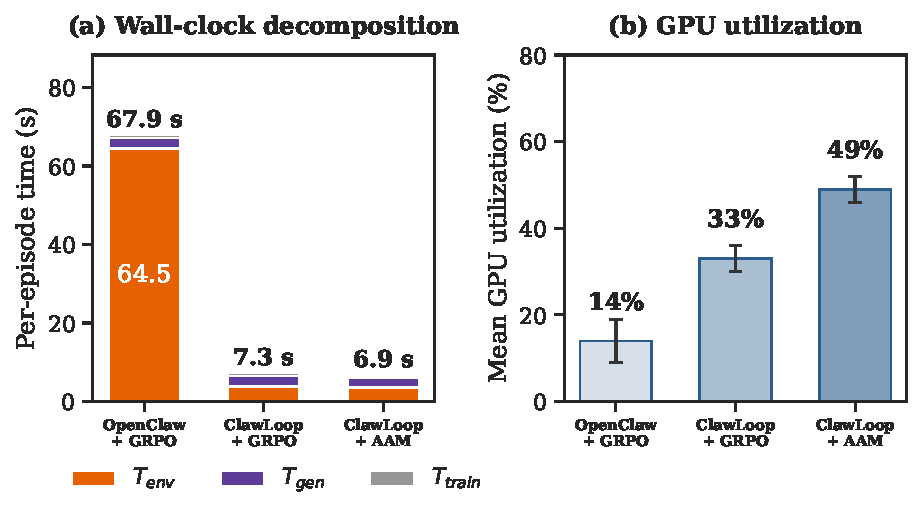
\includegraphics[width=0.9\linewidth]{fig_train_eff.pdf}
    \caption{
    Training-side efficiency.
    (a) Per-episode wall-clock time decomposition.
    (b) Mean GPU utilization.
    ClawLoop drastically reduces environment overhead, while AAM further improves efficiency by minimizing redundant interactions.
    }
    \label{fig:train_eff}
\end{figure}


\begin{figure*}[th]
  \centering
  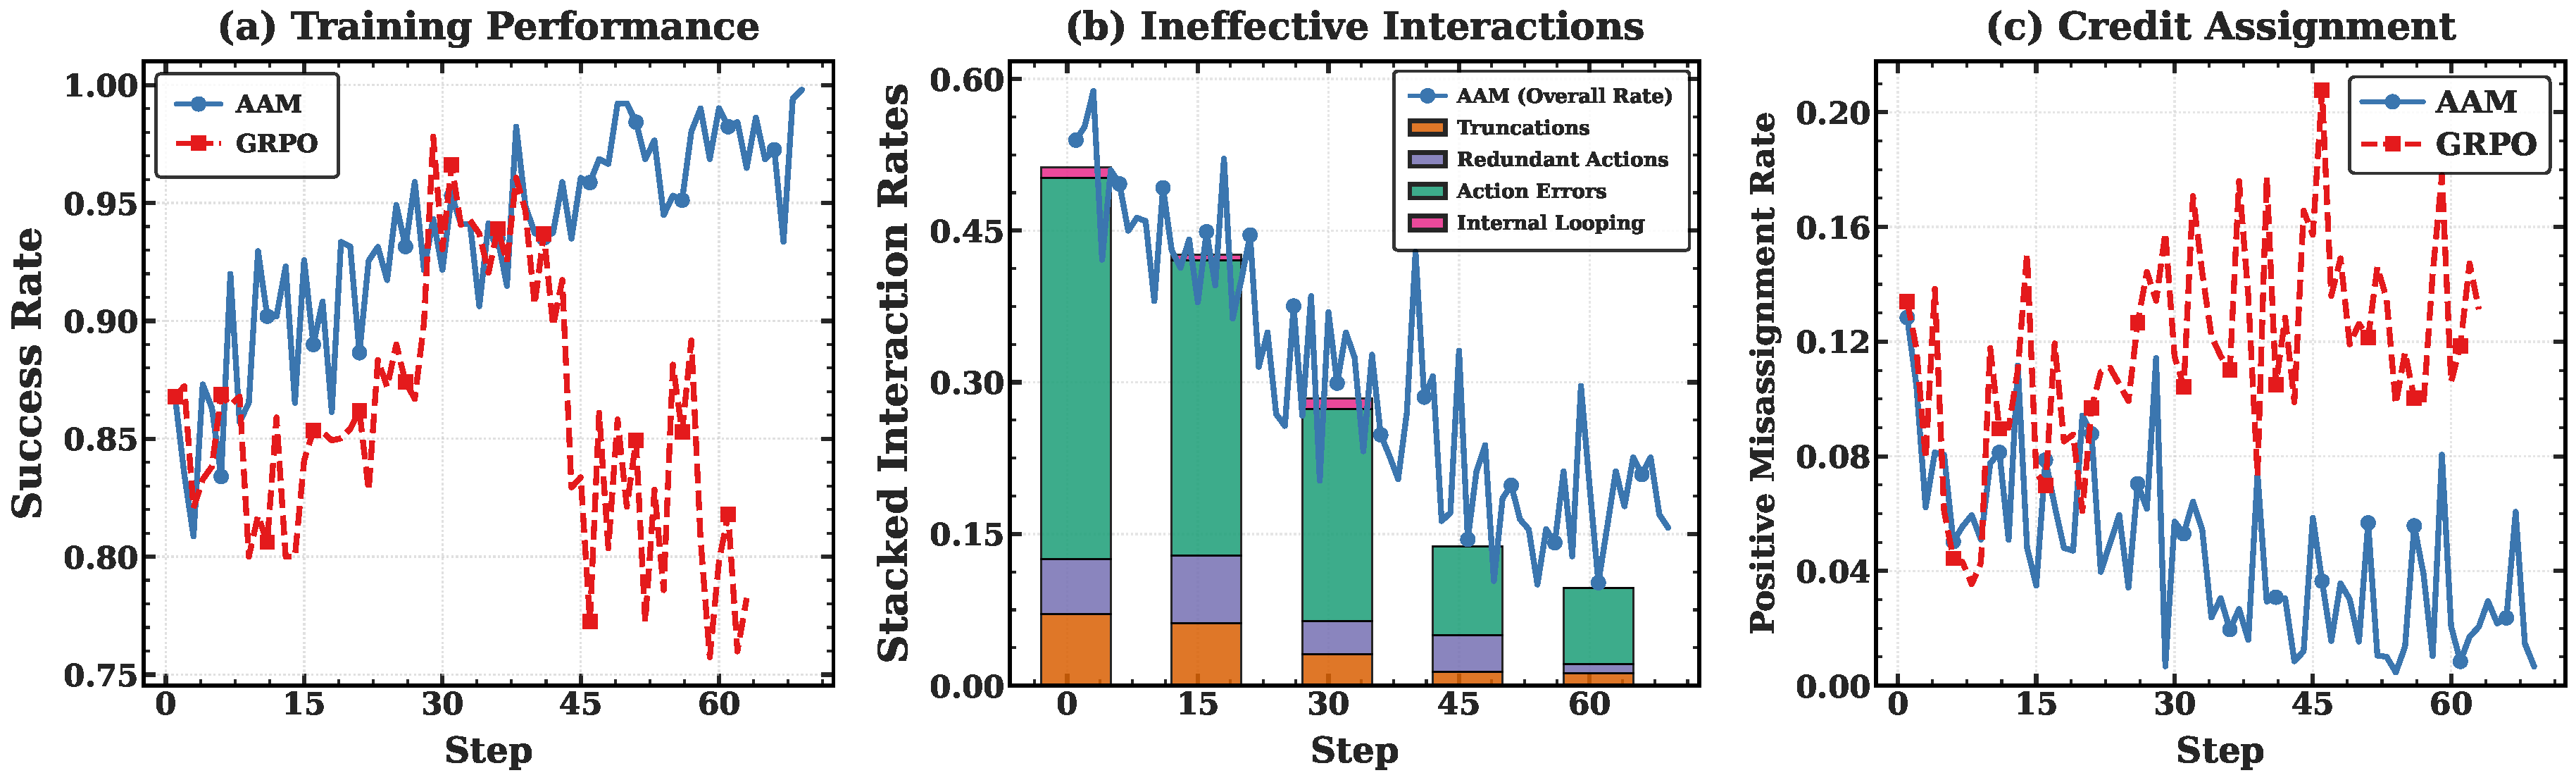
\includegraphics[width=0.8\textwidth]{./grpo_three_figures_combined-Copy1.pdf}
    \caption{
    Training dynamics of GRPO vs.\ AAM on Qwen3.5-9B.
    (a) Success rate $\bar p(t)$ for GRPO and AAM;
    (b) Stacked ineffective-interaction rates $r_{\mathrm{inv}}(t)$; 
    % decomposed into internal looping, redundant actions, truncations, and action errors.
    (c) Positive-gradient misassignment $\psi_+(t)$(occurred in GRPO vs. prevented by AAM).
    % AAM suppresses the post-peak rise of ineffective interactions and keeps positive reinforcement concentrated on productive tokens.
    % Shaded bands denote 95\% bootstrap confidence intervals.
    }
  \label{fig:dynamics}
\end{figure*}


\subsection{Efficiency Analysis}
\label{subsec:efficiency}
% P1: 训练效率，柱状图分析，三个对比。
% P2: 推理效率侧 token-acc(SR) 相关曲线，对比Base model 系统，我们的训练模型，几个api-LLM
\paragraph{Training-side efficiency.}
We compare three training configurations under identical settings: OpenClaw in-harness GRPO, ClawLoop with GRPO, and ClawLoop with AAM.
As shown in Fig.~\ref{fig:train_eff}(a), the product-level harness remains dominated by environment execution, costing $64.5\,\mathrm{s}$ per episode.
ClawLoop reduces this to $7.3\,\mathrm{s}$, achieving a $8.8\times$ speedup by stripping non-essential components from the rollout path.
Notably, AAM further cuts per-episode time to $6.9\,\mathrm{s}$, as suppressing ineffective interactions shortens average trajectory length.
This reduction in wasted computation translates to higher efficiency: mean GPU utilization increases from $14\%$ (OpenClaw) to $33\%$ (ClawLoop + GRPO), and further to $49\%$ with AAM (Fig.~\ref{fig:train_eff}(b)).
These results demonstrate that eliminating ineffective interactions is critical for improving GPU utilization, as it minimizes idle time caused by redundant environment feedback and unnecessary token generation.
% These results show that the efficiency gain comes primarily from the lightweight harness, while AAM improves learning quality without materially increasing training cost.

\paragraph{Inference-side efficiency.}
We further examine whether the efficiency gain persists at test time.
Fig.~\ref{fig:token_sr} plots success rate against average token consumption per episode.
For each model family, we show results from 2B to 27B parameters.
The base Qwen3.5 models improve as scale increases, but still consume a large number of tokens while achieving moderate success rates, indicating that many generated steps do not contribute to task completion.
After training with ClawLoop and AAM, our models at every scale move toward the lower-right region: they achieve higher success rates while using fewer tokens.
This gap widens at larger scales: Qwen3.5-27B with AAM reaches \textbf{66.4}\% SR with only \textbf{5.7K} tokens per episode, approaching GPT-5 (\textbf{67.2}\% SR) while using substantially fewer tokens.
The result suggests that AAM does not merely improve accuracy; it produces more efficient agent behavior by reducing ineffective interaction steps.

\begin{figure}[th]
    \centering
    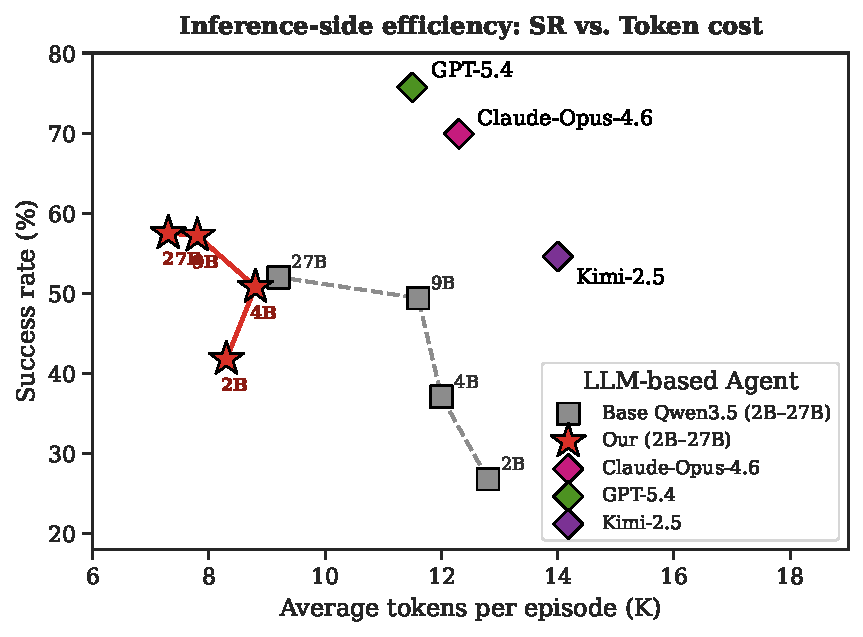
\includegraphics[width=0.8\linewidth]{fig_token_sr.pdf}
    \caption{
    Inference-side efficiency. Success rate as a function of average token consumption per episode.
    % Our AAM-trained model achieves competitive success rate with fewer tokens than the base model and proprietary API-based LLMs.
    }
    \label{fig:token_sr}
\end{figure}




\subsection{Training Dynamics}
\label{subsec:dynamics}
Here, we compare the training dynamics of standard GRPO and AAM on Qwen3.5-9B under the same setting as in Section \S\ref{subsec:prelim_misassign}.
Fig.~\ref{fig:dynamics} reports three curves:
(a) success rate $\bar p(t)$,
(b) ineffective-interaction rate $r_{\mathrm{inv}}(t)$, and
(c) positive-gradient misassignment $\psi_+(t)$.
% Both runs use the same evaluation schedule and the same ineffective-interaction detector as in the preliminary analysis (\S\ref{subsec:prelim_misassign}).

% GRPO reproduces the collapse pattern observed earlier: $\bar p(t)$ first rises to a peak and then declines, while $r_{\mathrm{inv}}(t)$ increases in anti-phase and $\psi_+(t)$ grows from $\approx\!0.11$ to $\approx\!0.53$.
AAM substantially alters the collapse behavior during training.
Its success rate continues to improve after the GRPO collapse point and stabilizes at a higher plateau, with no sustained post-peak degradation.
Meanwhile, $r_{\mathrm{inv}}(t)$ remains low, and $\psi_+(t)$ stays near its early-training level, indicating that positive reinforcement no longer accumulates on ineffective tokens.
% The small residual $\psi_+$ under AAM mainly comes from imperfect detection and boundary tokens whose effectiveness is ambiguous.
These curves suggest that GRPO collapse arises because successful but inefficient episodes reinforce ineffective tokens along with productive ones.
AAM breaks this feedback loop by masking positive advantage on ineffective tokens, concentrating learning on actions that advance the task, yielding more stable training and a higher success rate.

% \begin{figure*}[th]
%   \centering
%   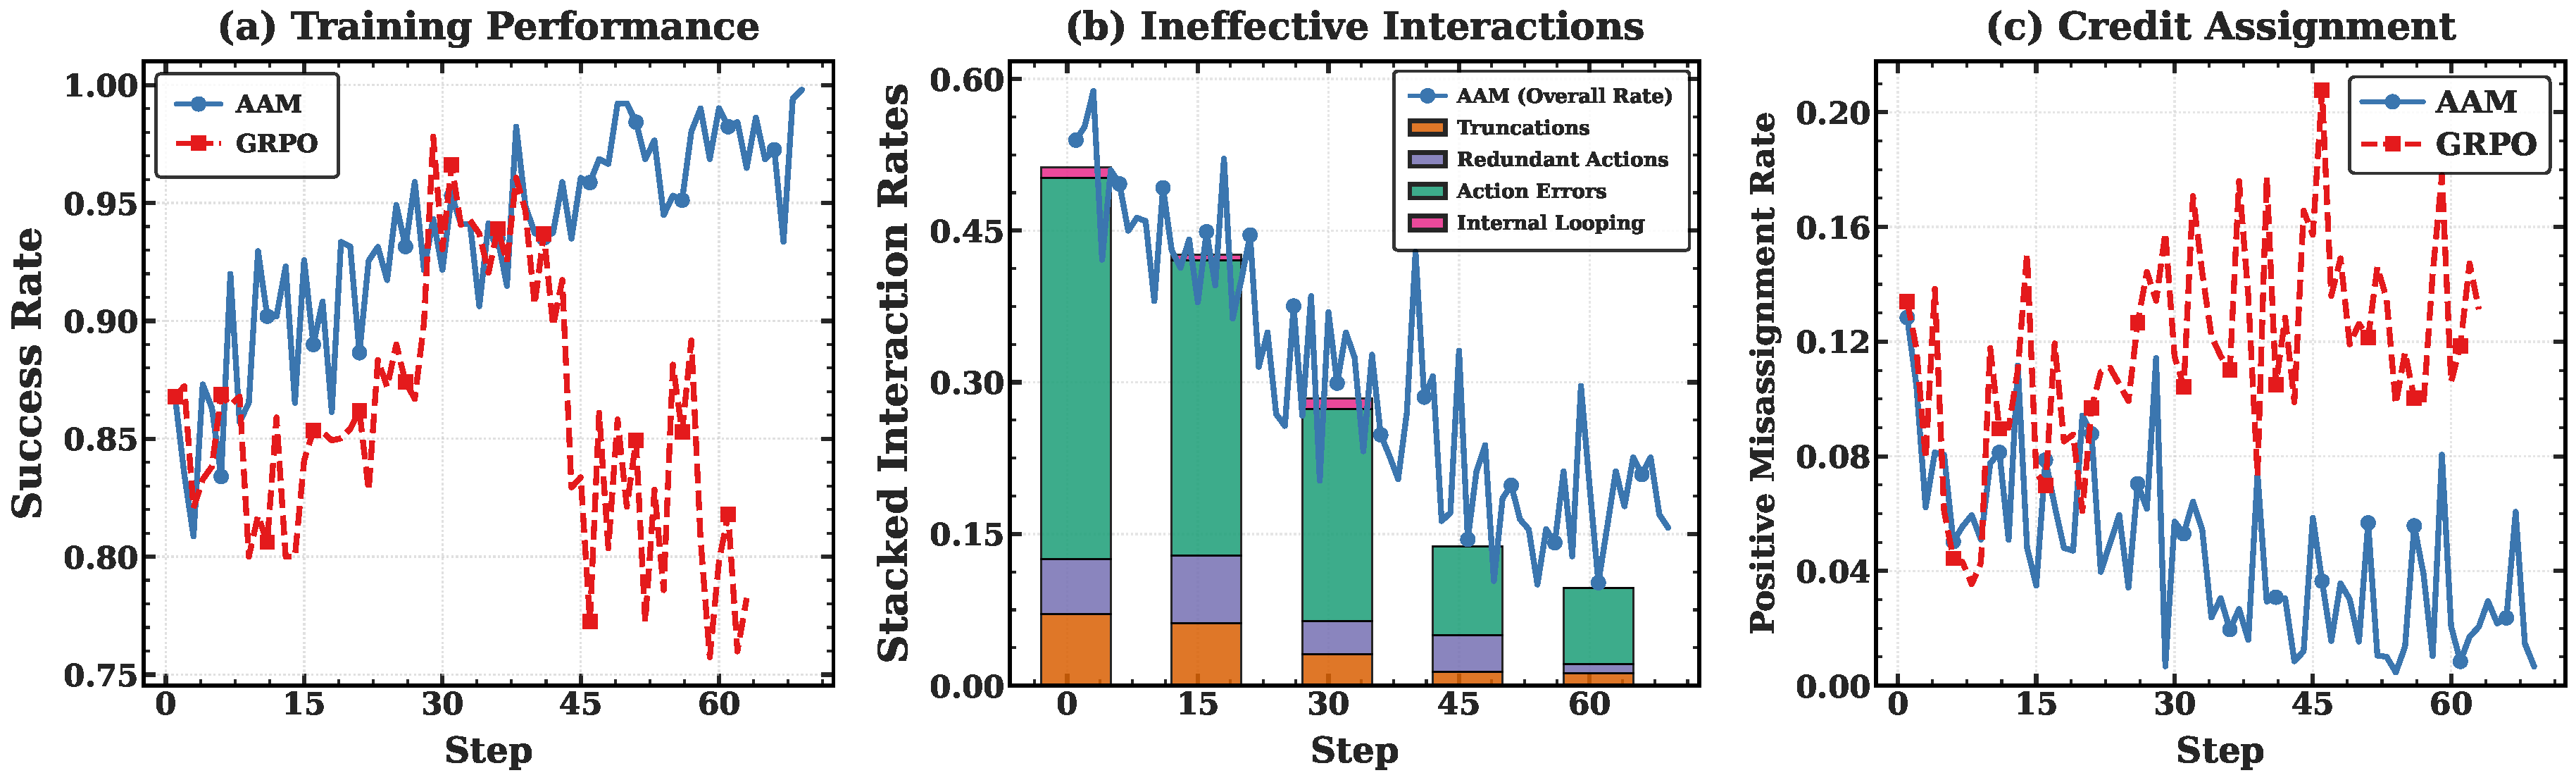
\includegraphics[width=0.8\textwidth]{./grpo_three_figures_combined-Copy1.pdf}
%     \caption{
%     Training dynamics of GRPO vs.\ AAM on Qwen3.5-9B.
%     (a) Success rate $\bar p(t)$ for GRPO and AAM;
%     (b) Stacked ineffective-interaction rates $r_{\mathrm{inv}}(t)$; 
%     % decomposed into internal looping, redundant actions, truncations, and action errors.
%     (c) Positive-gradient misassignment $\psi_+(t)$.
%     % AAM suppresses the post-peak rise of ineffective interactions and keeps positive reinforcement concentrated on productive tokens.
%     % Shaded bands denote 95\% bootstrap confidence intervals.
%     }
%   \label{fig:dynamics}
% \end{figure*}


\subsection{Ablation Study}
\label{subsec:ablation}
To isolate AAM's gains, we conduct ablations on Qwen3.5-9B and report average PinchBench success rate in Table~\ref{tab:ablation}.
% Unless otherwise specified, all variants are trained for the same number of steps and evaluated under the same protocol.

\paragraph{Each ineffective-pattern mask contributes.}
Disabling any single pattern mask reduces performance.
The largest drops come from removing masks for redundant actions and action errors ($-4.10$ and $-3.80$ SR), indicating that these tokens are especially harmful when they receive positive reinforcement in otherwise successful trajectories.
The masks for internal looping and truncation produce smaller but consistent effects ($-0.30$ and $-0.40$ SR).
This result is broadly consistent with the training-dynamics analysis in \S\ref{subsec:prelim_misassign}: redundant interactions directly waste valid turns, while action errors provide explicit failure signals that should not be positively reinforced.

\paragraph{Asymmetric masking is essential.}
Symmetric masking, which zeros gradients on ineffective tokens regardless of advantage sign, underperforms full AAM by $6.30$ SR.
This shows that simply removing gradient signal from ineffective tokens is insufficient.
AAM suppresses only \emph{positive} reinforcement on ineffective tokens while preserving \emph{negative} advantage, allowing the policy to learn avoidance rather than merely forgetting the corresponding behavior.

\paragraph{The gain is not due to random gradient sparsification.}
Random masking, which zeros the same fraction of tokens uniformly at random, trails full AAM by $5.50$ SR and does not recover AAM's improvement.
This rules out generic regularization or reduced gradient mass as the main source of gain: the benefit depends on identifying ineffective tokens and applying advantage-asymmetric masking to them.

\begin{table}[t]
    \centering
    % \small
    \begin{tabular}{lcc}
        \toprule
        Variant & Avg.\ SR & $\Delta$ \\
        \midrule
        AAM (full)              & \textbf{57.20} & -- \\
        \midrule
        \quad w/o Looping       & 56.90 & $-0.30$ \\
        \quad w/o Redundant     & 53.10 & $-4.10$ \\
        \quad w/o Truncation    & 56.80 & $-0.40$ \\
        \quad w/o Error         & 53.40 & $-3.80$ \\
        \midrule
        Symmetric masking       & 50.90 & $-6.30$ \\
        Random masking          & 51.70 & $-5.50$ \\
        \bottomrule
    \end{tabular}
    \caption{
    Ablation of AAM on Qwen3.5-9B.
    Avg.\ SR (\%) is the average in-domain success rate.
    $\Delta$ denotes the change.
    }
    \vspace{-6pt}
    \label{tab:ablation}
\end{table}


% \section{Conclusion}
% We identify environment overhead and credit misassignment as two fundamental bottlenecks in in-harness agent RL, and address them through ClawLoop and Asymmetric Advantage Masking.
% ClawLoop strips product-level complexity to achieve an faster speedup in environment execution, while AAM corrects token-level credit assignment to eliminate training collapse.
% Experiments demonstrate consistent gains in both training stability and inference efficiency.
% These results establish that practical in-harness RL requires co-designing lightweight execution infrastructure and fine-grained optimization signals.

\section{Conclusion}
We identify environment overhead and credit misassignment as two bottlenecks in in-harness RL, addressing them through ClawLoop and Asymmetric Advantage Masking.
ClawLoop strips product complexity for faster environment execution, while AAM corrects token-level credit assignment, eliminating training collapse.
Experiments show consistent gains in training stability and inference efficiency.
These results show that practical in-harness RL requires co-designing lightweight infrastructure and fine-grained optimization signals.


% \section*{Acknowledgments}
% AAAI is especially grateful to Peter Patel Schneider for his work in implementing the original aaai.sty file, liberally using the ideas of other style hackers, including Barbara Beeton. We also acknowledge with thanks the work of George Ferguson for his guide to using the style and BibTeX files.

\bibliography{aaai2027}

% Check whether the conference requires a reproducibility checklist to be included in the paper.
% If so, you can uncomment the following line and ajust the path to include it.
% \input{ReproducibilityChecklist.tex}

\end{document}
